\section{Analysis of loop hierarchy}\label{Sec:Stoflo}

In this section, we prove Theorem \ref{lem:main_ind}. The argument largely follows that in Section 5 of \cite{YY_25}, except for Section \ref{subsection-sum-zero}, which requires the main new inputs of this paper. However, even for the estimates before Section \ref{subsection-sum-zero}, there are a lot of technical power-countings that are dimension-dependent. (For example, the $E_{a}$ matrices in \eqref{Def_matE} have a factor of $W^{2}$ with exponent matching the dimension. Also, the ball of radius $\ell$ in $\Z_{L}^{2}$ has size $O(\ell^{2})$. These changes are reflected in the definition of $M_{t}$ from \eqref{eq:bcal_k}, and it is important to keep track of them carefully.) For this reason, unless the argument is identical to the corresponding argument in \cite{YY_25} at the level of power-counting, we will provide details for proofs.

\subsection{Proof of Theorem \ref{lem:main_ind}: Step 1}

\begin{proof}
We recall that the goal of this first step is to prove \eqref{lRB1} and \eqref{Gtmwc}. First, we use the assumption $t\leq1-N^{-1+\tau}$ in Theorem \ref{lem:main_ind} and the definitions \(\ell_t = \ell(z_t)\) and \(\eta_t = \im z_t\). This gives
$$
1 - u \gg N^{-1}, \quad \eta_u \gg N^{-1}, \quad u \le t.
$$
Given that \(\partial_z (H - z)^{-1} = (H - z)^{-2}\) and that the entries of \(H_t\) are jointly Gaussian, we deduce that for any \(C > 0\), there exists \(C'\) such that the following is true outside of events whose probabilities are exponentially small in $N$:
\begin{equation}\label{Gopboundu}
    \max_{u:\,1-u \ge N^{-1}} \max_{|u - u'| \leq N^{-C'}} \| G_u - G_{u'} \|_{\max} \leq N^{-C}.
\end{equation}
Hence, by a standard net argument, it suffices to prove \eqref{lRB1} and \eqref{Gtmwc} for \(u = t\). This continuity argument will be used repeatedly in this paper. 

\paragraph{Case 1: \(s < t \leq 1/2\).} 
We have $\|G_{t}\|_{op}\leq1/\eta_{t}=O(1)$. We also have \(\|E_a\|_{op} \leq W^{-2}\) for all \(a \in \mathbb{Z}_L^{2}\). Thus,  
\begin{equation}\label{Lboundfor1/2}
    {\cal L}_{t, \boldsymbol{\sigma}, \textbf{a}} = \left\langle \prod_{i=1}^n G_t(\sigma_i) E_{a_i} \right\rangle = O(W^{-2(n-1)}), \quad t \leq 1/2.
\end{equation}
Since $M_{t}=W^{2}\ell_{t}^{2}\eta_{t}=O(W^{2})$ for $t\leq1/2$, the bound \eqref{Lboundfor1/2} implies \eqref{lRB1}. Next, we combine \eqref{Lboundfor1/2} with \eqref{GijGEX} and \eqref{GiiGEX}, and we note that $\ell_{t},\eta_{t}$ are order $1$ for $t\leq1/2$. This gives
$$
{\bf 1}\left(\|G_t - m\|_{\max} \leq W^{-1/10}\right) \cdot \|G_t - m\|_{\max} \prec W^{-1}, \quad t \leq 1/2.
$$
By \eqref{Gopboundu} and the previous display, we deduce that $\|G_{u}-m\|_{\max}\prec W^{-1}$ implies $\|G_{u'}-m\|_{\max}\prec W^{-1}$ for any $|u'-u|\leq N^{-C'}$ if $C'>0$ is large enough. Thus, as soon as we can find a single time $u_{0}\in[s,t]$, where $t\leq1/2$, such that $\|G_{u_{0}}-m\|_{\max}\prec W^{-1}$, we would deduce this bound for all $u\in[s,t]$. By \eqref{Gt_bound+IND}, we can choose $u_{0}=s$, and thus \eqref{Gtmwc} holds, i.e.
\begin{equation}\label{Gtmt12}
    \|G_u - m\|_{\max} \prec W^{-1}, \quad u \leq 1/2.
\end{equation}

\paragraph{Case 2: \(t > s \geq 1/2\).} 
By \eqref{eq:bcal_k} from Lemma \ref{ML:Kbound}, we have ${\cal K}_{s, \boldsymbol{\sigma}, \textbf{a}} \prec M_{s}^{-n+1}$, where we recall $M_{s}=W^{2}\ell_{s}^{2}\eta_{s}$. If we combine this with the assumption \eqref{Eq:L-KGt+IND}, then we get that for any fixed \(n\) and \(s\), 
\begin{equation}\label{Lboundfors}
    {\cal L}_{s, \boldsymbol{\sigma}, \textbf{a}}\prec M_{s}^{-n+1}.
\end{equation}
We now record the following estimate, whose proof follows from the same argument as in Section 6 of \cite{YY_25}. {An outline of the proof is given in Section \ref{sec:Inh_LE}.}



\begin{lemma}\label{lem_ConArg}
Suppose that \(c < t_1 \leq t_2 \leq 1\) for some constant \(c > 0\). Assume that for any fixed \(n\geq1\), the following bounds hold at time \(t_1\): 
\begin{equation}\label{55}
    \max_{\boldsymbol{\sigma}, \textbf{a}} {\cal L}_{t_1, \boldsymbol{\sigma}, \textbf{a}} \prec M_{t_{1}}^{-n+1},\quad M_{t}:=W^{2}\ell_{t}^{2}\eta_{t}.
\end{equation}
Next, we let $\Omega$ denote the following event:
\begin{equation}\label{usuayzoo}
    \Omega := \left\{\|G_{t_2}\|_{\max} \leq 2\right\}.
\end{equation}
Then, for any fixed \(n \geq 1\), we have
\begin{equation}\label{res_lo_bo_eta}
    {\bf 1}_\Omega \cdot \max_{\boldsymbol{\sigma}, \textbf{a}} {\cal L}_{t_2, \boldsymbol{\sigma}, \textbf{a}} \prec (W^{2}\ell_{t_{1}}^{2}\eta_{t_{2}})^{-n+1} = \left( \frac{\ell_{t_{2}}}{\ell_{t_{1}}} \right)^{2(n-1)} \cdot M_{t_{2}}^{-n+1}.
\end{equation}
\end{lemma}

By \eqref{Lboundfor1/2} and \eqref{Lboundfors}, the a priori bound \eqref{55} for \({\cal L}_s\) holds. Thus, we can use Lemma \ref{lem_ConArg} to obtain
\begin{equation}\label{jsajufua}
    {\bf 1}\left(\|G_{u}\|_{\max} \leq 2\right) \cdot \max_{\boldsymbol{\sigma}, \textbf{a}} {\cal L}_{u, \boldsymbol{\sigma}, \textbf{a}} \prec \left( \frac{\ell_u}{\ell_s} \right)^{2(n-1)} \cdot M_{u}^{-n+1}, \quad s \leq u \leq t.
\end{equation}
Now, we use \eqref{jsajufua} for $n=2$ with Lemma \ref{lem_GbEXP} gives us
$$
{\bf 1}\left(\|G_u - m\|_{\max} \leq M_{u}^{-1/6}\right) \cdot \|G_u - m\|_{\max} \prec \frac{\ell_u}{\ell_s} \cdot M_{u}^{-1/2}, \quad s \leq u \leq t.
$$
By \eqref{con_st_ind}, we know $\ell_{u}\ell_{s}^{-1}\leq M_{s}^{1/60}$. Combining this with the previous display, we deduce that for any $D>0$, we have the following for $N$ large enough:
\begin{equation}
    \mathbb{P}\left(M_{u}^{-1/4} \leq \|G_u - m\|_{\max} \leq M_{u}^{-1/6}\right) \leq N^{-D}, \quad s \leq u \leq t.
\end{equation}
Another standard continuity argument (e.g. \eqref{Gopboundu}) allows us to insert either a maximum or minimum over $u\in[s,t]$ in the event above. 

Now, by assumption, we have the initial data bound $\|G_s - m\|_{\max} \prec M_{s}^{-1/2}$. Together with the previous display and continuity of $G_{u}$ in $u$, we deduce $\|G_t - m\|_{\max} \prec M_{t}^{-1/4}$. Combining this bound with \eqref{jsajufua} gives \eqref{lRB1} and \eqref{Gtmwc} for $t>s\geq1/2$.

\paragraph{Case 3: \(t > 1/2 > s\).} From Case 1, we know that \eqref{Lboundfor1/2} and \eqref{Gtmt12} hold for \(t = 1/2\). The proof of Case 2 uses only these two conditions. Thus, the current case follows as a consequence of Case 2 with \(s = 1/2\).
\end{proof}



\subsection{Dynamics of  \texorpdfstring{$\cal L-\cal K$}{L-K}}

 Recall the loop hierarchy from Lemma \ref{lem:SE_basic}. We now introduce the notation
$$
\mathcal{L}_{t,\;  \mathcal{G}^{(a), \,L}_{k, \,l}\left(\boldsymbol{\sigma},\, \textbf{a}\right)} := \left( \mathcal{G}^{(a), L}_{k, l} \circ \mathcal{L}_{t, \boldsymbol{\sigma}, \textbf{a}} \right), \quad  
\mathcal{L}_{t,\;  \mathcal{G}^{(b), \,R}_{k, \,l}\left(\boldsymbol{\sigma},\, \textbf{a}\right)} := \left( \mathcal{G}^{(b), R}_{k, l} \circ \mathcal{L}_{t, \boldsymbol{\sigma}, \textbf{a}} \right),
$$
which allows us write the hierarchy in a more convenient form that we describe below. By (5.15) in \cite{YY_25}, we have the following equation, which uses notation to be clarified afterwards:
\begin{align}\label{eq_L-Keee}
    d(\mathcal{L} - \mathcal{K})_{t, \boldsymbol{\sigma}, \textbf{a}} = &
    \Big[\mathcal{K} \sim (\mathcal{L} - \mathcal{K})\Big]^{l_\mathcal{K} = 2}_{t, \boldsymbol{\sigma}, \textbf{a}}dt + \sum_{l_\mathcal{K} > 2} \Big[\mathcal{K} \sim (\mathcal{L} - \mathcal{K})\Big]^{l_\mathcal{K}}_{t, \boldsymbol{\sigma}, \textbf{a}}dt + \mathcal{E}^{((\mathcal{L} - \mathcal{K}) \times (\mathcal{L} - \mathcal{K}))}_{t, \boldsymbol{\sigma}, \textbf{a}} +
    \mathcal{E}^{(M)}_{t, \boldsymbol{\sigma}, \textbf{a}} +
    \mathcal{E}^{(\widetilde{G})}_{t, \boldsymbol{\sigma}, \textbf{a}}.
\end{align} 
Above, the last two terms are introduced in Lemma \ref{lem:SE_basic}. The first two terms are defined by the formula
\begin{align}\label{DefKsimLK}
&\; W^{2}\cdot \sum_{1 \leq k < l \leq n} \sum_{a, b}  
   \Big( 
   (\mathcal{L} - \mathcal{K})_{t,\;  \mathcal{G}^{(a), \,L}_{k, \,l}\left(\boldsymbol{\sigma},\, \textbf{a}\right)} 
   \cdot S^{(B)}_{ab}
   \cdot 
   \mathcal{K}_{t,\;  \mathcal{G}^{(b), \,R}_{k, \,l}\left(\boldsymbol{\sigma},\, \textbf{a}\right)} \cdot \textbf{1}(\text{length of $\mathcal{K}$ equals } l_\mathcal{K})   \nonumber \\
   & + \left(\mathcal{K} \iff \mathcal{L-K} \right) \Big) 
    := \sum_{l_{\cal K}=2}^n\Big[\mathcal{K} \sim (\mathcal{L} - \mathcal{K})\Big]^{l_\mathcal{K}}_{t, \boldsymbol{\sigma}; \textbf{a}},
\end{align}
here, \( \mathcal{K} \iff \mathcal{L-K} \) denotes the terms obtained by swapping \(\mathcal{K}\) and \(\mathcal{L-K}\). Next, we introduce
\begin{equation}\label{def_ELKLK}
    \mathcal{E}^{((\mathcal{L} - \mathcal{K}) \times (\mathcal{L} - \mathcal{K}))}_{t, \boldsymbol{\sigma}, \textbf{a}} :=
    W^{2}\cdot\sum_{1 \leq k < l \leq n} \sum_{a, b} (\mathcal{L} - \mathcal{K})_{t,\;  \mathcal{G}^{(a), \,L}_{k, \,l}\left(\boldsymbol{\sigma},\, \textbf{a}\right)} \cdot  S^{(B)}_{ab} \cdot (\mathcal{L} - \mathcal{K})_{t,\;  \mathcal{G}^{(b), \,R}_{k, \,l}\left(\boldsymbol{\sigma},\, \textbf{a}\right)} \, dt.
\end{equation}

We will turn \eqref{eq_L-Keee} into an integral equation. First, we introduce the main objects in this integral equation construction.


\begin{definition}\label{DefTHUST}
Define the linear map ${\varTheta}_{t, \boldsymbol{\sigma}}$ via the following action on a tensor ${\cal A}: \mathbb Z^n_L\to \mathbb C$: 
\begin{align}
    \left({{\varTheta}}_{t, \boldsymbol{\sigma}} \circ \mathcal{A}\right)_{\textbf{a}} & = \sum_{i=1}^n \sum_{b_i} \left(\frac{m_i m_{i+1} S^{(B)} }{1 - t m_i m_{i+1} S^{(B)}}\right)_{a_i b_i} \cdot \mathcal{A}_{\textbf{a}^{(i)}},\quad m_i=m(\sigma_i) \nonumber \\
    \quad \textbf{a}^{(i)}&  = (a_1, \ldots, a_{i-1}, b_i, a_{i+1}, \ldots, a_n).
\end{align}  
We also define the semigroup operator $\mathcal{U}_{s,t,\boldsymbol{\sigma}}$ associated to $\Theta_{t,\boldsymbol{\sigma}}$ as follows
    \begin{align}\label{def_Ustz}
        \left(\mathcal{U}_{s, t, \boldsymbol{\sigma}} \circ \mathcal{A}\right)_{\textbf{a}} = \sum_{b_1, \ldots, b_n} \prod_{i=1}^n \left(\frac{1 - s \cdot m_i m_{i+1} S^{(B)}}{1 - t \cdot m_i m_{i+1} S^{(B)}}\right)_{a_i b_i} \cdot \mathcal{A}_{\textbf{b}}, \quad \textbf{b} = (b_1, \ldots, b_n), \quad m_i=m(\sigma_i)
    \end{align}
\end{definition}
Note that for any $\xi \in \mathbb{C}$, we have the following identity:
 \begin{align}\label{def_Ustz_2}
\left(\frac{1 - s \xi S^{(B)}}{1 - t \xi S^{(B)}}\right) = I - (s - t) \xi \cdot \Theta^{(B)}_{t \xi} \cdot S^{(B)}.
\end{align}
By the explicit formula \eqref{Kn2sol} for ${\cal K}$ of rank $2$, the first term on the right-hand side of \eqref{eq_L-Keee} can be rewritten as $({\varTheta}_{t, \boldsymbol{\sigma}} \circ (\mathcal{L} - \mathcal{K}))_{\textbf{a}} = [\mathcal{K} \sim (\mathcal{L} - \mathcal{K})]^{l_\mathcal{K} = 2}_{t, \boldsymbol{\sigma}, \textbf{a}}$. Using this and the Duhamel principle, we have the following.


\begin{lemma}[Integrated loop hierarchy] 
    \label{Sol_CalL}
For any $t\geq0$, we have the SDE
%
\begin{align}\label{LK_SDE}
d({\cal L}-{\cal K})_{t,\boldsymbol{\sigma},\textbf{a}}=(\varTheta_{t,\boldsymbol{\sigma}}\circ({\cal L}-{\cal K})_{t,\boldsymbol{\sigma},\cdot})_{\textbf{a}}dt+\sum_{l_\mathcal{K} > 2} \Big[\mathcal{K} \sim (\mathcal{L} - \mathcal{K})\Big]^{l_\mathcal{K}}_{t, \boldsymbol{\sigma}, \textbf{a}}dt + \mathcal{E}^{((\mathcal{L} - \mathcal{K}) \times (\mathcal{L} - \mathcal{K}))}_{t, \boldsymbol{\sigma}, \textbf{a}} +
    \mathcal{E}^{(M)}_{t, \boldsymbol{\sigma}, \textbf{a}} +
    \mathcal{E}^{(\widetilde{G})}_{t, \boldsymbol{\sigma}, \textbf{a}}.
\end{align}
%    
For any $s<t$, we have the following ``integrated" loop hierarchy:
\begin{align}\label{int_K-LcalE}
    (\mathcal{L} - \mathcal{K})_{t, \boldsymbol{\sigma}, \textbf{a}} \;=\; \; &
    \left(\mathcal{U}_{s, t, \boldsymbol{\sigma}} \circ (\mathcal{L} - \mathcal{K})_{s, \boldsymbol{\sigma}}\right)_{\textbf{a}} \nonumber \\
    &+ \sum_{l_\mathcal{K} > 2} \int_{s}^t \left(\mathcal{U}_{u, t, \boldsymbol{\sigma}} \circ \Big[\mathcal{K} \sim (\mathcal{L} - \mathcal{K})\Big]^{l_\mathcal{K}}_{u, \boldsymbol{\sigma}}\right)_{\textbf{a}} du \nonumber \\
    &+ \int_{s}^t \left(\mathcal{U}_{u, t, \boldsymbol{\sigma}} \circ \mathcal{E}^{((\mathcal{L} - \mathcal{K}) \times (\mathcal{L} - \mathcal{K}))}_{u, \boldsymbol{\sigma}}\right)_{\textbf{a}} du  \nonumber \\
    &+ \int_{s}^t \left(\mathcal{U}_{u, t, \boldsymbol{\sigma}} \circ \mathcal{E}^{(\widetilde{G})}_{u, \boldsymbol{\sigma}}\right)_{\textbf{a}} du + \int_{s}^t \left(\mathcal{U}_{u, t, \boldsymbol{\sigma}} \circ \mathcal{E}^{(M)}_{u, \boldsymbol{\sigma}}\right)_{\textbf{a}}  
\end{align}
Furthermore, let $T\geq s$ be a stopping time with respect to the matrix Brownian motion $H_t$ and set $\tau:= T\wedge t$. We have the stopped integrated loop hierarchy below for any $t\geq s$:
\begin{align}\label{int_K-L_ST}
   (\mathcal{L} - \mathcal{K})_{\tau , \boldsymbol{\sigma}, \textbf{a}} \;=\; \; &
    \left(\mathcal{U}_{s, \tau, \boldsymbol{\sigma}} \circ (\mathcal{L} - \mathcal{K})_{s, \boldsymbol{\sigma}}\right)_{\textbf{a}}  \nonumber \\
    &+ \sum_{l_\mathcal{K} > 2} \int_{s}^\tau \left(\mathcal{U}_{u, \tau, \boldsymbol{\sigma}} \circ \Big[\mathcal{K} \sim (\mathcal{L} - \mathcal{K})\Big]^{l_\mathcal{K}}_{u, \boldsymbol{\sigma}}\right)_{\textbf{a}} du  \nonumber \\
    &+ \int_{s}^\tau \left(\mathcal{U}_{u, \tau, \boldsymbol{\sigma}} \circ \mathcal{E}^{((\mathcal{L} - \mathcal{K}) \times (\mathcal{L} - \mathcal{K}))}_{u, \boldsymbol{\sigma}}\right)_{\textbf{a}} du  \nonumber \\
    &+ \int_{s}^\tau \left(\mathcal{U}_{u, \tau, \boldsymbol{\sigma}} \circ \mathcal{E}^{(\widetilde{G})}_{u, \boldsymbol{\sigma}}\right)_{\textbf{a}} du + \int_{s}^\tau \left(\mathcal{U}_{u, \tau, \boldsymbol{\sigma}} \circ \mathcal{E}^{(M)}_{u, \boldsymbol{\sigma}}\right)_{\textbf{a}}.
\end{align}

 %$$
 %\left({\cal U}_{\tau, t}\right)^{-1}\circ\int_s^\tau\left(\mathcal{U}_{u, t, \boldsymbol{\sigma}} \circ \mathcal{E}^{(M)}_{u, \boldsymbol{\sigma}}\right)_{\textbf{a}} ,\quad \left( {\cal U}_{\tau, t}\right)^{-1}={\cal U}_{t,\tau}$$
 
\end{lemma}

The last term in \eqref{int_K-L_ST} has the following meaning. Since ${\cal U}$ is deterministic, the object obtained by replacing ${\cal U}_{u,\tau,\boldsymbol{\sigma}}$ by ${\cal U}_{u,t,\boldsymbol{\sigma}}$ is well-defined, and this object is continuous in $t$, so we can evaluate it at time $t=\tau$. Of course, one must be careful in using It\^{o} calculus to estimate it.

We now introduce notation that is necessary to compute the quadratic variation of the martingale.

 
\begin{definition}[Definition of $\mathcal{E}\otimes  \mathcal{E}$]\label{def:CALE} 
Denote 
  \begin{align}\label{defEOTE}
 \left( \mathcal{E}\otimes  \mathcal{E} \right)_{t, \,\boldsymbol{\sigma}, \,\textbf{a}, \,\textbf{a}'} \; := \; &
 \sum_{k=1}^n\left( \mathcal{E}\otimes  \mathcal{E} \right)^{(k)}_{t, \,\boldsymbol{\sigma}, \,\textbf{a}, \,\textbf{a}'}
 \nonumber \\
 \left( \mathcal{E}\otimes  \mathcal{E} \right)^{(k)}_{t, \,\boldsymbol{\sigma}, \,\textbf{a}, \,\textbf{a}'} :
\; = \; & W^{2} \sum_{b,b'} S^{(B)}_{b,b'}{\cal L}_{t, \boldsymbol{\sigma}^{(k ) },\textbf{a}^{(k )}},\quad \boldsymbol{\sigma}^{(k ) }\in \{+,-\}^{2n+2}, 
\end{align}
where ${\cal L}_{t, \boldsymbol{\sigma}^{(k ) },\textbf{a}^{(k )}}$ is obtained by cutting the $k$-th edge of ${\cal L}_{t,\boldsymbol{\sigma},\textbf{a}}$ and then attaching itself (with indices $\textbf{a}$) to its complex conjugate loop (with indices $\textbf{a}'$) into a bigger loop that is labeled by indices $b$ and $b'$, so that
%where $\textbf{a}^{(k )}(m)$ is the $m$-th component of $\textbf{a}^{(k )}$. More precisely
\begin{align}\label{def_diffakn_k}
   & \textbf{a}^{(k )}=( a_k,a_{k+1},\cdots a_n, a_1,\cdots a_{k-1}, b', a'_{k-1}\cdots a_1', a_n'\cdots a'_{k},b)
    \nonumber \\
  &  \boldsymbol{\sigma}^{(k )}=( \, \sigma_k, \, \sigma_{k+1},\cdots \sigma_n,  \, \sigma_1,\cdots \sigma_{k}, \,  \overline\sigma_{k},  \cdots \overline\sigma_1 , \,  \overline\sigma_n \cdots \overline\sigma_{k })
\end{align}
The symbol $\otimes$ is used to emphasize the symmetric structure of $\mathcal{E} \otimes \mathcal{E}$; it is not a tensor product.  


 
 

\begin{figure}[ht]
\centering
\begin{minipage}{0.45\textwidth} % Adjust width as needed
    \centering
    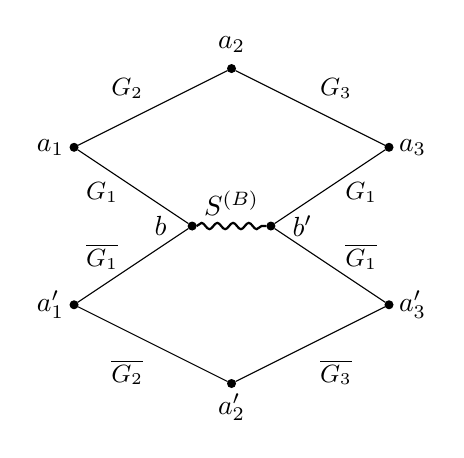
\begin{tikzpicture}[scale=1.0]

    % Define nodes with visible dots for origin
    \node[draw, circle, inner sep=1pt, fill=black] (A1) at (-2, 2) {};
    \node at (-2.3, 2) {$a_1$}; % Offset label above

    \node[draw, circle, inner sep=1pt, fill=black] (A2) at (0, 3) {};
    \node at (0 , 3.3) {$a_2$}; % Offset label to the right

    \node[draw, circle, inner sep=1pt, fill=black] (A3) at (2, 2) {};
    \node at (2.3, 2 ) {$a_3$}; % Offset label above

    \node[draw, circle, inner sep=1pt, fill=black] (B) at (-0.5, 1) {};
    \node at (-0.9, 1) {$b$}; % Offset label to the left

    \node[draw, circle, inner sep=1pt, fill=black] (B1) at (0.5, 1) {};
    \node at (0.9, 1) {$b'$}; % Offset label to the right

    \node[draw, circle, inner sep=1pt, fill=black] (A1b) at (-2, 0) {};
    \node at (-2.3, -0) {$a'_1$}; % Offset label below

    \node[draw, circle, inner sep=1pt, fill=black] (A2b) at (0, -1) {};
    \node at (0, -1.3) {$a'_2$}; % Offset label to the right

    \node[draw, circle, inner sep=1pt, fill=black] (A3b) at (2, 0) {};
    \node at (2.3, -0) {$a'_3$}; % Offset label below

    % Draw connections (upper diamond)
    \draw (A1) -- (A2) node[midway, above left] {\small $G_2$}; % Reduced font size
    \draw (A2) -- (A3) node[midway, above right] {\small $G_3$}; % Reduced font size
    \draw (A1) -- (B) node[midway, below left, xshift=-2pt, yshift= 5pt] {\small $G_1$}; % Adjusted position
    \draw (A3) -- (B1) node[midway, below right, xshift=2pt, yshift= 5pt] {\small $G_1$}; % Adjusted position

    % Draw connections (lower diamond)
    \draw (B) -- (A1b) node[midway, above left,  xshift=-2pt, yshift=-5pt] {\small $\overline{G_1}$}; % Reduced font size
    \draw (A1b) -- (A2b) node[midway, below left, yshift=-2pt] {\small $\overline{G_2}$}; % Adjusted position
    \draw (A2b) -- (A3b) node[midway, below right, yshift=-2pt] {\small $\overline{G_3}$}; % Adjusted position
    \draw (B1) -- (A3b) node[midway, above right, xshift=2pt, yshift=-5pt] {\small $\overline{G_1}$}; % Adjusted position

    % Connect b and b' with a wavy line and add "S" label
    \draw[decorate, decoration={snake, amplitude=0.4mm, segment length=2mm}, thick] (B) -- (B1)
        node[midway, above] {$S^{(B)}$};

    \end{tikzpicture}
   
\end{minipage}%
\hfill
\begin{minipage}{0.45\textwidth} % Adjust width as needed
    \raggedright
     % Adjust vertical alignment as needed
    $$k=1 $$\\ 
    $$\textbf{a}^{(1 )}=( a_1, a_2, a_3, b', a_3', a_2', a_1',b);$$
    \\  
     $$\boldsymbol{\sigma}^{(1 )}=(\;\sigma_1, \sigma_2, \sigma_3,\sigma_1, \overline{\sigma_1},\overline{\sigma_3}, \overline{\sigma_2},\overline{\sigma_1}, ).$$
\end{minipage}
 \caption{Example of the $8-G$ loop in $\mathcal{E}\otimes  \mathcal{E}$: for $\sigma\in \{+,-\}^3$. Taken from \cite{YY_25}.}
    \label{fig:8shapedgraph}
\end{figure}


\end{definition}

 We now estimate the martingale term in \eqref{int_K-L_ST} via Lemma 5.5 in \cite{YY_25}, which we record below.

\begin{lemma}\label{lem:DIfREP}
For any stopping time $T$ with respect to the filtration generated by $H_t$ we have
 \begin{equation}\label{alu9_STime}
   \mathbb{E} \left [    \int_{s}^\tau\left(\mathcal{U}_{u, t, \boldsymbol{\sigma}} \circ \mathcal{E}^{(M)}_{u, \boldsymbol{\sigma}}\right)_{\textbf{a}} \right ]^{2p} 
   \le C_{n,p} \; 
   \mathbb{E} \left(\int_{s}^\tau 
   \left(\left(
   \mathcal{U}_{u, t,  \boldsymbol{\sigma}}
   \otimes 
   \mathcal{U}_{u, t,  \overline{\boldsymbol{\sigma}}}
   \right) \;\circ  \;
   \left( \mathcal{E} \otimes  \mathcal{E} \right)
   _{u, \,\boldsymbol{\sigma}  }
   \right)_{{\textbf a}, {\textbf a}}du 
   \right)^{p}
  \end{equation} 
  where $\tau:=t\wedge T$, where  $\overline{\boldsymbol{\sigma}}$ is the conjugate of ${\boldsymbol{\sigma}}$, and where
  $$
  \left[\left(
   \mathcal{U}_{u, t,  \boldsymbol{\sigma}}
   \otimes 
   \mathcal{U}_{u, t,  \overline{\boldsymbol{\sigma}}}
   \right)\circ \cal A\right]_{\textbf{a},\textbf{a}'}=
   \sum_{\textbf{b},\;\textbf{b}'} \; \prod_{i=1}^n \left(\frac{1 - u \cdot m_i m_{i+1} S^{(B)}}{1 - t \cdot m_i m_{i+1} S^{(B)}}\right)_{a_i b_i}
   \;\cdot \;\prod_{i=1}^n \left(\frac{1 - u \cdot \overline{m_i m_{i+1}} S^{(B)}}{1 - t \cdot \overline{m_i m_{i+1}} S^{(B)}}\right)_{a'_i b'_i} \cdot \mathcal{A}_{\textbf{b},\textbf{b}'}.
  $$
\end{lemma}



 
  




\subsection{Proof of Theorem \ref{lem:main_ind}, Step 2}
In this subsection, we will fix $\boldsymbol{\sigma}=(+,-)$ and thus drop it from the notation.  We prove \eqref{Eq:Gdecay_w} first;  \eqref{Gt_bound_flow} will be proved at the end of this  section. 
We start by defining the following exponential decay profiles:
\begin{equation}\label{def_WTu}
      {\cal T}^{(\cal L-K)}_u (\ell):= \max_{a,\,b\; : \; |a-b|\ge \ell} \left| ({\cal L-K})_{u,  \boldsymbol{\sigma},  ( a, b)}\right|,\quad  \boldsymbol{\sigma}=(+,-),
\end{equation}
\begin{equation}\label{def_WTuD}
{\cal T} _{u, D} (\ell) := M_{u}^{-2}
\exp \left(- \left( \ell /\ell_u \right)_+^{1/2} \right)+W^{-D}.
\end{equation} 
Both  ${\cal T}^{(\cal L-K)}_u$ and ${\cal T} _{u, D}$ are non-increasing in the parameter $\ell$, so for any $0\leq\ell_{1}\leq\ell_{2}$, we have 
 ${\cal T}^{(\cal L-K)}_u (\ell_1)\ge {\cal T}^{(\cal L-K)}_u (\ell_2)$ and ${\cal T} _{u,D} (\ell_1)\ge{\cal T} _{u,D}(\ell_2)$. We will denote the ratio between \eqref{def_WTu} and \eqref{def_WTuD} by  % (the plus 1 is for the simplicity of future argument).
\begin{equation}\label{def_Ju}
     {\cal J} _{u,D} (\ell):=   \left({\cal T}^{(\cal L-K)}_u (\ell) \Big/{\cal T}_{u,D} (\ell)\right)+1
\end{equation} 
Our goal is to control $ {\cal J} _{u,D} (\ell)$ for any $u\in [s,t]$ and any large $D>0$. In particular, we aim to show 
 \begin{align}\label{shoellJJ}
    {\cal J}^* _{u,D} :=\max_{\ell}   {\cal J} _{u,D} (\ell)\prec (\eta_s/\eta_u)^4 
  \end{align}
In this subsection, we will often use the following slightly enlarged length-scale:
$$
  \ell^{*}_t := (\log W)^{3/2}\cdot \ell_t .
$$
In this scale $\ell_t^*$,  $\Theta_t$ is exponentially small, but ${\cal T}_t$ is not. 
More precisely, we have the following lemma, which is Lemma 5.6 in \cite{YY_25}. (The proof is identical to that of Lemma 5.6 in \cite{YY_25}, so we omit it. In any case, the first and third estimates below are elementary, and the last follows by decay of ${\cal K}$, which follows from the explicit formula \eqref{Kn2sol}, decay of $\Theta$ from \eqref{prop:ThfadC}, and decay of ${\cal L}-{\cal K}$.)
\begin{lemma}\label{lem_dec_calE_0}
For any fixed $D,\delta>0$, we have
 \begin{align}
 \label{Kell*}
   |b -a|_{L}\ge \delta \cdot \ell_t^* &\implies 
   \left({\Theta}_t\right)_{ab } \le W^{-D} ,\quad    \left({\Theta}_s^{-1}{\Theta}_t\right)_{ab } \le W^{-D}
   \\
  |b -a|_{L}\ge \delta \cdot \ell_t^* 
 & \implies  {\cal L}_{t, (+,-),(a, b)} \prec {\cal J}^*_{t,D}\cdot{\cal T}_{t,D}(|a-b|_{L}) . \label{auiwii}
\end{align}
Moreover, for any $C=O(1)$, we have \begin{equation}\label{Tell*}
       { {\cal T}_{u,D} \left(\ell-C\cdot \ell_u^*\right)}\;\prec \;  {\cal T}_{u,D} \left(\ell \right).
\end{equation} 

\end{lemma}




Our proof of \eqref{Eq:Gdecay_w} relies on the loop hierarchy \eqref{int_K-L_ST} for $n=2$. 
We begin by bounding  terms in \eqref{int_K-L_ST}.  

\begin{lemma}\label{lem_dec_calE}  Suppose  the assumptions of Theorem  \ref{lem:main_ind} and the conclusion  of Step 1, i.e., \eqref{lRB1} and \eqref{Gtmwc}, 
hold. Assume that the following are satisfied, in which $\textbf{a}=(a_{1},a_{2})$ and $\textbf{a}'=(a_{1}',a_{2}')$ and $\boldsymbol{\sigma}=(+,-)$:
\begin{align} 
s\le u\le t, \quad  D\ge D_{0}, \quad 
\max_i |a_i-a_i'|_{L}\le \ell_t ^*. \label{57}
\end{align}
Here $D_{0}=D_{0}(\mathfrak{c})$ is a sufficiently large constant (in the proof, the term $W^{-D}$ in ${\cal T}_{u,D}$ is summed over at most $N^{O(1)}\leq W^{O(1/\mathfrak{c})}$ indices). Then we have
\begin{align}\label{res_deccalE_lk}
       {\cal E}^{( (L-K)\times(L-K) )}
       _{u, \boldsymbol{\sigma},\textbf{a}} \Big/\; 
  {\cal T}_{t,D}(|a_1-a_2|_{L}) \quad 
 \;  &\; \prec \; 
   \left(\eta_u\right)^{-1} 
   \cdot  
   M_{u}^{-1}
    \cdot 
 \left({\cal J}^{*}_{u,D} \right)^{2}
 \\
      \mathcal{E}^{( \widetilde{G} )}_{u, \boldsymbol{\sigma},\textbf{a}} 
    \;\Big/\; 
 {\cal T}_{t,D}(|a_1-a_2|_{L})
 \;  &\; \prec \; 
 \left(\eta_u\right)^{-1} 
  \cdot \left(\ell_u/\ell_s\right)^{4}\cdot{\bf 1}(|a_1-a_2|_{L}\le \ell_u^*)
    \nonumber  \\
       \;  &\; + \;  \left(\eta_u\right)^{-1} 
  \cdot
       \left(M_{u}^{-1/2}  \cdot 
       \left({\cal J}^{*}_{u,D} \right)^{2}+M_{u}^{-3/2}  \cdot 
       \left({\cal J}^{*}_{u,D} \right)^{3}\right)
 \label{res_deccalE_wG}\\
\label{res_deccalE_dif}
    \left(
   \mathcal{E}\otimes  \mathcal{E} \right)
   _{u, \,\boldsymbol{\sigma},  \,{\textbf a} ,\, {\textbf a}'
     }
     \;\Big/\; 
 \left( {\cal T}_{t,D}(|a_1-a_2|_{L})\right)^2
 \;  &\; \prec \; 
  \left(\eta_u\right)^{-1} 
  \cdot \left(\ell_u/\ell_s\right)^{10}\cdot{\bf 1}(|a_1-a_2|_{L}\le 4\ell_t^*)
     \nonumber \\
       \;  &\; + \;  \left(\eta_u\right)^{-1} 
  \cdot\left(\ell_u/\ell_s\right)^{3}\cdot
       M_{u}^{-1/2}  \cdot 
    \left({\cal J}^{*}_{u,D} \right)^{2}
     \nonumber \\
       \;  &\; + \;\left(\eta_t\right)^{-1} 
  \cdot
       M_{t}^{-1}  \cdot 
    \left({\cal J}^{*}_{u,D} \right)^{3}
\end{align} 
  \end{lemma}


Assuming  Lemma \ref{lem_dec_calE}, we now  prove  \eqref{Eq:Gdecay_w}. We will extensively use the estimates for $\cal U$ from Section \ref{ks}. 


\begin{proof}[Proof of \eqref{Eq:Gdecay_w}]
By  assumption \eqref{Eq:Gdecay+IND} on $({ \cal L-\cal K})_s$, the operator norm bound on $\cal U$ in Lemma \ref{lem:sum_Ndecay},  and the  tail estimate  \eqref{neiwuj}, 
%of Lemma \ref{TailtoTail}, 
we can  bound the first term on the right side  of \eqref{int_K-L_ST} by 
\begin{equation} \label{res_deccalE_0}
\left(\mathcal{U}_{s, t, \boldsymbol{\sigma}} \circ (\mathcal{L} - \mathcal{K})_{s, \boldsymbol{\sigma}}\right)_{\textbf{a}}\;\Big/\; 
  {\cal T}_{t, D}(|a_1-a_2|_{L}) \quad 
  \prec \;   (\ell_t/\ell_s)^{4}\cdot {\bf 1}(|a_1-a_2|_{L}\le \ell_t^*) + 1,
\end{equation}
where the last term of order one comes from applying \eqref{neiwuj}. The factor $\left(\eta_s / \eta_t\right)^2$  from applying Lemma \ref{lem:sum_Ndecay} becomes 
$ (\ell_t/\ell_s)^{4}$ due to the prefactors in $ {\cal T}_{s, D}$ and  ${\cal T}_{t, D}$.
For  any $\textbf{a}$ fixed and any function $f$,  we decompose $f  = f (\textbf{b}) {\bf 1} ( \| \textbf{b}-\textbf{a}\|\le \ell_t^*)  + f_2   $. 
From the decay of ${\cal U}_{u,t}$,  we know that $( {\cal U}_{u,t, \boldsymbol{\sigma}} \circ f_2 )_\textbf{a}$ is exponentially small.  
Hence we only have to bound $  {\cal U}_{u,t, \boldsymbol{\sigma}} \circ f_1$, for which we apply  Lemma \ref{lem:sum_Ndecay}. Ultimately, for the third  term of \eqref{int_K-L_ST}, we have the following estimate, in which $\|\textbf{b}-\textbf{a}\|:=\max_{i}|b_{i}-a_{i}|_{L}$:
$$
 \Big({\cal U}_{u,t, \boldsymbol{\sigma}}\circ  {\cal E}^{( (L-K)\times(L-K) )}_{u, \boldsymbol{\sigma}}\Big)_\textbf{a}
 \prec (\eta_u/\eta_t)^2 \max_{\| \textbf{b}-\textbf{a}\|\le \ell_t^*}{\cal E}^{( (L-K)\times(L-K) )}_{u, \boldsymbol{\sigma}, \textbf{b}}+W^{-D}.
$$
Because we restrict to $\|\textbf{b}-\textbf{a}\|\leq\ell_{t}^{*}$, \eqref{Tell*} implies $ {\cal T}_{t, D}(|b_1-b_2|_{L})\prec  {\cal T}_{t, D}(|a_1-a_2|_{L})$. Thus, to control the right-hand side of the previous estimate, we can use the estimate \eqref{res_deccalE_lk} and closeness of $s,t$ in \eqref{con_st_ind} to get 
\begin{align} 
\label{res_deccalE_1}
     \Big({\cal U}_{u,t, \boldsymbol{\sigma}}\circ  {\cal E}^{( (L-K)\times(L-K) )}_{u, \boldsymbol{\sigma}}\Big)_\textbf{a}\;\Big/\; 
 {\cal T}_{t, D}(|a_1-a_2|_{L}) \quad 
  & \prec \; 
  \frac{1}{\eta_u}\left(\eta_u / \eta_t\right)^2 
   \cdot  
   M_{u}^{-1 }
    \cdot 
\left({\cal J}^*_{u,D}\right)^2
\end{align} 
Similarly,   the estimate \eqref{res_deccalE_wG} on ${\cal E}^{(\widetilde{G} )}$ implies   
\begin{align}  \label{res_deccalE_2}
     \Big(\mathcal{U}_{u,t, \boldsymbol{\sigma}} \circ  \mathcal{E}^{( \widetilde{G} )}_{u, \boldsymbol{\sigma}}\Big)_{\mathbf{a}} 
    \;\Big/\; 
{\cal T}_{t, D}(|a_1-a_2|_{L})
 &\prec \;  {\bf1}(|a_1-a_2|_{L}\le 3\ell_t^*)\cdot  \frac{1} {\eta_u} \cdot \left(\eta_u / \eta_t\right)^2\cdot \left(\ell_u / \ell_s\right)^4 
 \nonumber \\
  &+\;    \frac{1}{\eta_u} 
  \cdot\left(\eta_u / \eta_t\right)^2 \cdot
      M_{u}^{-1/2}  \cdot \left({\cal J}^{*}_{u,D} \right)^{2 }
 \nonumber \\
  &+\;    \frac{1}{\eta_u} 
  \cdot\left(\eta_u / \eta_t\right)^2 \cdot M_{u}^{-3/2}  \cdot \left({\cal J}^{*}_{u,D} \right)^{3 }, 
       \end{align} 
and  the  estimate  \eqref{res_deccalE_dif} on $\cal E\otimes\cal E$  implies  
\begin{align} \label{res_deccalE_3}
  \left(\left(
   \mathcal{U}_{u, t,  \boldsymbol{\sigma}}
   \otimes 
   \mathcal{U}_{u, t,  \overline{\boldsymbol{\sigma}}}
   \right) \;\circ  \;
   \left( \mathcal{E} \otimes  \mathcal{E} \right)
   _{u, \,\boldsymbol{\sigma}  }
   \right)_{{\textbf a}, {\textbf a}}
     \;\Big/\; 
 \left({\cal T}_{t, D}(|a_1-a_2|_{L})\right)^2
 &\prec \;  {\bf1}(|a_1-a_2|_{L}\le 6\ell_t^*)\cdot  \frac{1} {\eta_u} \cdot \left(\eta_u / \eta_t\right)^4\cdot \left(\ell_u / \ell_s\right)^{10} 
 \nonumber \\
 &+ \;  \left(\eta_u / \eta_t\right)^4\cdot\frac{1}{\eta_u} 
  \cdot\left(\ell_u / \ell_s\right)^{3}\cdot
       M_{u}^{-1/2}  \cdot \left({\cal J}^{*}_{u,D} \right)^{2 }
 \nonumber \\
 &+ \;\left(\eta_u / \eta_t\right)^4\cdot\frac{1}{\eta_t} 
  \cdot
       M_{t}^{-1}  \cdot \left({\cal J}^{*}_{u,D} \right)^{3 }.
\end{align}
We now insert  these bounds  into the stopped equation \eqref{int_K-L_ST} with $\tau:=T\wedge t$, where, for a fixed and sufficiently small $\delta>0$,
\begin{align}
T:=\min \{u\geq s: {\cal J}^*_{u,D} \ge N^{\delta}\left(\eta_s / \eta_t\right)^4\}
\end{align}
(If we divide each estimate in Lemma \ref{lem_dec_calE} by its right-hand side, the resulting estimates all hold with probability $1-O(N^{-D})$ for any $D>0$ simultaneously for all $u\in[s,t]$. This follows by another continuity argument.) With this stopping time, the quadratic variation of the martingale in \eqref{int_K-L_ST} is bounded as follows:
\begin{align}\label{51}
& \int_s^\tau  \left( \left(\mathcal{U}_{u,t,  \boldsymbol{\sigma}}
   \otimes 
   \mathcal{U}_{u, t,  \overline{\boldsymbol{\sigma}}}
   \right) \;\circ  \;
   \left( \mathcal{E}\otimes  \mathcal{E} \right)
   _{u, \,\boldsymbol{\sigma},\, \overline{\boldsymbol{\sigma}} }
   \right)_{{\textbf a}, {\textbf a}}  d u
 \Big/{\cal T}_{t, D}(|a_1-a_2|_{L})^2  \nonumber \\
 \prec  &   \int_s^\tau   d u \Big \{ 
 {\bf1}(|a_1-a_2|_{L}\le 6\ell_t^*)\cdot  \frac{1} {\eta_u} \cdot \left(\eta_u / \eta_t\right)^4\cdot \left(\ell_u / \ell_s\right)^{10}
\nonumber \\
&\qquad\qquad+ \;  \left(\eta_u / \eta_t\right)^4\cdot\frac{1}{\eta_u} 
  \cdot\left(\ell_u / \ell_s\right)^{3}\cdot
       M_{u}^{-1/2}  \cdot \left({\cal J}^{*}_{u,D} \right)^{2 }+\left(\eta_u / \eta_t\right)^4\cdot\frac{1}{\eta_t} 
  \cdot
       M_{t}^{-1}  \cdot \left({\cal J}^{*}_{u,D} \right)^{3 }  \Big \}   \nonumber \\
\le  &   C \big [ (\eta_s/\eta_t)^{5}  \cdot {\bf 1}(|a_1-a_2|_{L}\le 6\ell_t^*)+1 \big ]
 \end{align}
To see the last inequality, set $r:=\eta_s/\eta_t$, and recall that $\eta_u=(1-u)\im m$ and that $M_{u}$ is comparable to $W^{2}\min(1,L^{2}(1-u))$. Hence $(\ell_u/\ell_s)^{2}\leq\eta_s/\eta_u$ and $M_s/M_u\leq\eta_s/\eta_u\leq r$ for $u\in[s,t]$, so that \eqref{con_st_ind} gives $M_u\geq M_t\geq M_s/r\geq r^{29}$. Moreover, $M_t\geq N^{c_0}$ for some $c_0>0$, by the assumption $t\leq1-N^{-1+\tau}$ and \eqref{Main_DEL_COND}. For the first term, we use $\int_s^t\eta_u^{-1}(\eta_u/\eta_t)^4(\eta_s/\eta_u)^5du=r^4(r-1)/\im m$. For the remaining terms, we use ${\cal J}^{*}_{u,D}\leq N^{\delta}r^4$ for $s\leq u<\tau$, which holds by definition of $T$, together with $\int_s^t\eta_u^{-1}(\eta_u/\eta_t)^4(\eta_s/\eta_u)^{3/2}du\leq Cr^4$ and $\int_s^t\eta_t^{-1}(\eta_u/\eta_t)^4du\leq Cr^5$. This bounds the remaining terms by $CN^{2\delta}r^{12}M_t^{-1/2}+CN^{3\delta}r^{17}M_t^{-1}\leq CN^{3\delta}M_t^{-5/58}$, which is at most $1$ if $\delta>0$ is small enough (depending on $c_0$).
Now, by Lemma \ref{lem:DIfREP} and the previous display, we deduce
%
\begin{align*}
\int_{s}^{\tau}\Big({\cal U}_{u,t,\boldsymbol{\sigma}}\circ{\cal E}^{(M)}_{u,\boldsymbol{\sigma}}\Big)_{\textbf{a}}\Big/{\cal T}_{t, D}(|a_1-a_2|_{L})\prec (\eta_{s}/\eta_{t})^{5/2}\mathbf{1}(|a_{1}-a_{2}|_{L}\leq6\ell_{t}^{*})+1. 
\end{align*}
% 
Because this bound holds at the level of stochastic domination, a union bound and a net argument lets us replace $t$ on the left-hand side by a supremum over $t'\in[s,t]$. In particular, we can evaluate it at $t'=\tau$. (We emphasize that the stochastic domination nature of the previous estimate is crucial for this argument.) Combining this  bound with  \eqref{res_deccalE_0}, \eqref{res_deccalE_1},   \eqref{res_deccalE_2}  and  \eqref{int_K-L_ST}, we have 
$$
\left({\cal L}-{\cal K}\right)_{\tau, \textbf{a}}\Big/{\cal T}_{t, D}(|a_1-a_2|_{L}) \prec   \big [ (\eta_s/\eta_t)^{5/2}  \cdot {\bf 1}(|a_1-a_2|_{L}\le 6\ell_t^*)+1 \big ], 
$$
where we used ${\cal J}^*_{s,D} \prec 1$ from \eqref{Eq:L-KGt+IND} and \eqref{Eq:Gdecay+IND}; in particular, because of the factor $N^{\delta}$ in the definition of $T$, we have $T>s$ with probability $1-O(N^{-D})$. (The integrals over $u\in[s,\tau]$ of the bounds \eqref{res_deccalE_1} and \eqref{res_deccalE_2} are estimated as in the proof of \eqref{51}: the term with the indicator is $\mathrm{O}_{\prec}((\eta_s/\eta_t)^{2})$, since $\int_s^t\eta_u^{-1}(\eta_u/\eta_t)^2(\eta_s/\eta_u)^2du=(\eta_s/\eta_t)^{2}\log(\eta_s/\eta_t)/\im m$, and the remaining terms are bounded by $CN^{3\delta}M_t^{-5/58}\leq1$.) By another continuity argument, the above estimate holds for all $t$ satisfying the constraint \eqref{con_st_ind} simultaneously with probability $1-O(N^{-D})$ for any $D>0$. In particular, it holds even at the random time $t=\tau$, which implies
\begin{align}\label{52}
 {\cal J}^*_{\tau,D}\prec     (\eta_s/\eta_t)^{5/2}  
\end{align}
 Since $(\eta_s/\eta_t)^{5/2}\leq N^{-\delta/2}\cdot N^{\delta}(\eta_s/\eta_t)^{4}$, we deduce 
${\mathbb P} (T\le t )\leq N^{-D}$ for any large $D>0$, and \eqref{Eq:Gdecay_w} follows.    
\end{proof}
 
 
 
 We note that the previous argument gives
\begin{align}\label{53}
\left({\cal L}-{\cal K}\right)_{t, \textbf{a}}\Big/{\cal T}_{t, D}(|a_1-a_2|_{L}) \prec   \big [ (\eta_s/\eta_t)^{5/2}  \cdot {\bf 1}(|a_1-a_2|_{L}\le 6\ell_t^*)+1 \big ].
\end{align}






 \begin{proof}[Proof of Lemma \ref{lem_dec_calE}]
 This argument is essentially the same as the proof of Lemma 5.7 in \cite{YY_25}, but we give the proof here because it is fairly long and technical, and because there are delicate power-countings that are dimension-dependent (as discussed at the beginning of this section).
 
 
\emph{Proof of \eqref{res_deccalE_lk}.}  
Recall the monotonicity property $u\leq t\Rightarrow\ell_{u}\leq \ell_{t}$, which itself implies $u\leq t\Rightarrow{\cal T}_{u,D}\leq{\cal T}_{t,D}$. By definition, we have
\begin{align} {\cal E}^{( ({\cal L-K})\times({\cal L-K}) )}_{u,  \boldsymbol{\sigma},  \textbf{a} }
= &W^{2}\sum_{b_1,b_2}({\cal L-K})_{u,
\boldsymbol{\sigma}, 
( a_1, b_1)
}
S^{(B)}_{b_1,b_2}
({\cal L-K})_{u,  \boldsymbol{\sigma},  ( b_2, a_2)}
\end{align}
By definition of $S^{(B)}$,  we can restrict the sum to $|b_1-b_2|_{L}\le 1$. Next, we use the elementary inequalities: 
$$
\int_{0 }^a\exp\left(-\sqrt{(a-x)}-\sqrt x+ \sqrt a\right)dx\le C\approx 6.12
\quad \text{ and } \quad 
\int_{0 }^\infty\exp\left({-\sqrt x}\right)dx=2.
$$
This gives $\sum_{x}{\cal T}_{u,D}(|a_{1}-x|_{L}){\cal T}_{u,D}(|a_{2}-x|_{L})\prec M_{u}^{-2}\ell_{u}^{2}{\cal T}_{u,D}(|a_{1}-a_{2}|_{L})$, where the factor of $M_{u}^{-2}$ comes from counting $M_{u}$ factors on each side of this identity using \eqref{def_WTuD}, and the factor of $\ell_{u}^{2}$ comes from re-scaling in $\ell$ of $\ell_{u}$ in \eqref{def_WTuD}. Therefore, we have the following, which implies \eqref{res_deccalE_lk}:
\begin{align}\nonumber
{\cal E}^{( ({\cal L-K})\times({\cal L-K}) )}_{u,  \boldsymbol{\sigma},  \textbf{a} }
\; \prec \;& W^{2} ({\cal J}_{u,D}^*) ^2\cdot 
\sum_{x }  {\cal T}_{u, \,D}(|a_1-x|_{L}) \cdot {\cal T}_{u, \,D}(|a_2-x|_{L})   
\\\label{mmxiaoxi}
\; \prec \;&
({\cal J}_{u,D}^*) ^2 \cdot 
 \eta_u^{-1}\cdot M_{u}^{-1}\cdot  {\cal T}_{u,D }(|a_1-a_2|_{L}) .
\end{align} 

 
\medskip
\noindent 
\emph{Proof of   \eqref{res_deccalE_wG}}.    By definition, we  have 
\begin{align}
 \max_{\textbf{a}}{\cal E}^{(\widetilde G)}_{u,  \boldsymbol{\sigma},  \textbf{a} }
 \prec W^{2} \sum_{b_1,b_2} \langle \widetilde G_u E_{b_1}\rangle\cdot S^{(B)}_{b_1,b_2}\cdot  {\cal L}_{u, (-,+,+),(a_1, b_2, a_2)}+c.c.,\quad \widetilde{G}=G-m
 \end{align}
Recall $\Xi^{({\cal L})}_{t,m}:=\max_{\boldsymbol{\sigma},\textbf{a}}|{\cal L}_{t,\boldsymbol{\sigma},\textbf{a}}|\cdot M_{t}^{m-1}\cdot\mathbf{1}(\boldsymbol{\sigma}\in\{+,-\}^{m})$. By \eqref{GavLGEX}, \eqref{def_WTu}, \eqref{def_WTuD}, \eqref{def_Ju}, and \eqref{shoellJJ}, we have 
$$
\langle \widetilde G_u E_{b_1}\rangle\prec \Xi^{(\cal L)}_{u,2}\cdot M_{u}^{-1}\prec  M_{u}^{-1}+ {\cal J}^*_{u,D}\cdot M_{u}^{-2}.
$$
Therefore 
 \begin{align}\label{jiizziy}
\max_{\textbf{a}}{\cal E}^{(\widetilde G)}_{u,  \boldsymbol{\sigma},  \textbf{a} } \prec \frac{1}{ \ell_u^{2}\eta_u} \cdot \sum_{b }   \left|{\cal L}_{u, (-,+,+),(a_1, b , a_2)}\right|(1+{\cal J}^*_{u,D}\cdot M_{u}^{-1})
\end{align}
Now, let us first restrict to the case  $|a_1-a_2|_{L}\le \ell_u^*$. Define 
$$
\ell_u^{**}:= \ell_u\cdot (\log W)^3=\ell^*_u\cdot (\log W)^{3/2}
$$
Note that  ${\cal T}_{u,D}(\ell_u^{**})\prec W^{-D}$. Now, consider $b$ in \eqref{jiizziy} such that $|b-a_1|_{L}\le  \ell_u^{**}$; there are $\prec(\ell_{u}^{**})^{2}\prec\ell_{u}^{2}$ many such indices since we are in dimension $2$. For this restricted summation, we use \eqref{lRB1} to bound the loops in \eqref{jiizziy}. This gives
\begin{align}\label{alkkj}
 \sum_{b }{\bf 1}\big(|b-a_1|_{L}\le  \ell_u^{** }\big)\cdot  \left|{\cal L}_{u, (-,+,+),(a_1, b , a_2)}\right|\prec (\ell_u/\ell_s)^{4}\cdot M_{u}^{-2} \cdot \ell_u^{2}.
\end{align}
We are left to handle indices $|b-a_1|_{L}\ge \ell_u^{**}$. For this, we use a simpler estimate 
 $$
 \left|{\cal L}_{u, (-,+,+),(a_1, b , a_2)}\right|\prec \max_{x_1\in {\cal I}_{a_1}^{(2)},y\in {\cal I}_{b}^{(2)}}|G_{x_1,y}|.
$$
Next, we use \eqref{GijGEX} to estimate the right-hand side of the previous display:
$$
\max_{x_1\in {\cal I}_{a_1}^{(2)},y\in {\cal I}_{b}^{(2)}}|G_{x_1,y}|\prec \sum_{a_1', b'}\left({\cal L}_{u,(+,-),{(b',a_1')}}\right)^{1/2}{\bf1}\left(|a'_1-a_1|_{L}\le 1, |b-b'|_{L}\le 1\right).
$$
Since $|b-a_1|\ge \ell_u^{** }$, by  \eqref{auiwii} and ${\cal T}_{u,D}(|a_1-b|_{L})\prec W^{-D}$, we have  
$$
{\cal L}_{u,(+,-),{(b',a_1')}} \prec {\cal J}^*_{u,D}\cdot W^{-D}.
$$
Therefore, the contribution from indices $b$ in \eqref{jiizziy} satisfying $|b-a_1|\ge  \ell_u^{** }$ part is negligible, i.e.
\begin{align}\label{alkkj2}
 \sum_{b }{\bf 1}\big(|b-a_1|\ge  \ell_u^{** }\big)\cdot  \left|{\cal L}_{u, (-,+,+),(a_1, b , a_2)}\right|\prec  {\cal J}^*_{u,D}\cdot W^{-D}. 
\end{align}
We will not track the contribution of the last term; it does not affect the argument given below. Now, since $|a_{1}-a_{2}|_{L}\leq\ell_{u}^{\ast}$, we know that ${\cal T}_{u,D}(|a_{1}-a_{2}|_{L})$ is bounded away from $0$; this follows by \eqref{Tell*}. Combining this with \eqref{alkkj} and  \eqref{jiizziy} gives the following, which implies the desired estimate \eqref{res_deccalE_wG} for $|a_1-a_2|_{L}\le \ell_u^*$:
\begin{align}\label{82jjdopasj}
 |a_1-a_2|\le \ell_u^*\implies  \mathcal{E}_{u, \boldsymbol{\sigma}, \mathbf{a}}^{(\widetilde{G})} \Big/{\cal T}_{u,D}(|a_1-a_2|_{L})\prec 
 (\eta_u)^{-1} \cdot \left(\ell_u / \ell_s\right)^4\cdot   \left(1+  (\mathcal{J}_{u, D}^*)^2  M_{u}^{-1 }\right).
 \end{align}

(Here we note that $(\ell_u/\ell_s)^{4}M_u^{-1}\leq M_u^{-1/2}$, since $(\ell_u/\ell_s)^{2}\leq\eta_s/\eta_u\leq M_s^{1/30}$ and $M_u\geq M_s^{29/30}$ by \eqref{con_st_ind}.) We now prove the desired estimate \eqref{res_deccalE_wG} under the assumption that $|a_1-a_2|\ge \ell_u^*$. For this, we consider the following two cases:
 $$
 (1): \min_i|a_i-b|\le \ell_u^*/2,\quad \quad 
 (2): \min_i|a_i-b|\ge \ell_u^*/2.
 $$
In the first case,  we assume without loss of generality that $|a_1-b|_{L}\le \ell_u^*/2$. Applying the Schwarz inequality to  the two $G$ edges  in ${\cal L}_{u, (-,+,+),(a_1, b , a_2)}$ connecting the block $a_2$ gives
$$
G_{x_1x_2}G_{x_2y}G_{yx_1}\prec |G_{x_1x_2}|^2|G_{yx_1}|+
|G_{ x_2 y}|^2|G_{yx_1}|.
$$
Therefore, we have
\begin{align}\label{kskjw}
  {\cal L}_{u, (-,+,+),(a_1, b , a_2)}
  \;\prec\; &\;  W^{-2} \Big ( {\cal L}_{u, (-,+),(a_1, a_2)} \ \max_{x_1\in {\cal I}^{(2)}_{a_1}}\sum_{y\in {\cal I}^{(2)}_{b}}|G_{x_1y}|+ {\cal L}_{u, (-,+),(a_2, b)}\ \max_{y\in {\cal I}^{(2)}_{b}}\sum_{x_1\in {\cal I}^{(2)}_{a_1}}|G_{x_1y}| \Big )  .
\end{align}
If we use \eqref{GijGEX},  the $\cal K$ bound and $\sqrt { 1+c } \le 1+c $, \eqref{def_WTu}, \eqref{def_WTuD}, \eqref{def_Ju}, and \eqref{shoellJJ},  we have
$$
{\bf 1}(x_1\ne x_2)|G_{x_1x_2}|\prec M_{u}^{-1/2}(1+{\cal J}^*_{u,D}M_{u}^{-1}).
$$
Thus, for any $a,b$, we have 
\begin{align}\label{jaysw2002}
  W^{-2}  \max_{y\in{\cal I}_b^{(2)}}\sum_{x\in{\cal I}_a^{(2)}}|G_{xy}|\prec M_{u}^{-1/2}(1+{\cal J}^*_{u,D}M_{u}^{-1})
\end{align}
Plugging this bound  into \eqref{kskjw} gives 
\begin{align}
  {\cal L}_{u, (-,+,+),(a_1, b , a_2)}
     \;\prec\; &\;\left( {\cal L}_{u, (-,+),(a_1, a_2)}   + {\cal L}_{u, (-,+),(a_2, b)}  \right)  \cdot M_{u}^{-1/2}(1+{\cal J}^*_{u,D}M_{u}^{-1})
\end{align}
 Since $|a_2-b|\ge \ell_u^*/2$ and $|a_1-a_2|\ge  \ell_u^*$,  we can estimate  $ {\cal L}_{u, (-,+),(a_1, a_2)}   + {\cal L}_{u, (-,+),(a_2, b)}$ 
with \eqref{auiwii} to have  
$$
 {\cal L}_{u, (-,+,+),(a_1, b , a_2)} \;\prec\; {\cal J}^*_{u,D}\cdot \left(  {\cal T}_{u,D}(|a_1-a_2|)+{\cal T}_{u,D}(|b-a_2|) \right)  \cdot M_{u}^{-1/2}(1+{\cal J}^*_{u,D}M_{u}^{-1})
 $$
Since $|b-a_2|_{L}\ge |a_1-a_2|_{L}-|a_1-b|_{L}\ge |a_1-a_2|_{L}-\ell_u^*/2$, we can use \eqref{Tell*} to deduce
$${\cal T}_{u,D}(|b-a_2|) \prec  {\cal T}_{u,D}(|a_1-a_2|)
$$
Combining these bounds along with bound ${\cal J}^{*}_{u,D}\geq1$ gives the following for $|a_1-a_2|_{L}\ge \ell_u^*$:
\begin{align}
    \label{lwjufw}
    \sum_{b } ^{\text{Case } 1} \left|{\cal L}_{u, (-,+,+),(a_1, b , a_2)}\right|\prec \left({\cal J}^*_{u,D}\right)^2\cdot{\cal T}_{u,D}(|a_1-a_2|_{L}) \cdot \ell_u^{2} M_{u}^{-1/2} .
\end{align}
We now consider case (2), defined below \eqref{82jjdopasj}. We bound  ${\cal L}_{u, (-,+,+),(a_1, b , a_2)}$ as follows
\begin{align}\label{LGGGXXX}
{\cal L}_{u, (-,+,+),(a_1, b , a_2)}
\prec \max_{x_1,x_2, y} \left|G_{x_1y}\right| \left|G_{yx_2}\right|\left|G_{x_1x_2}\right|{\bf 1}(x_1\in {\cal I}_{a_1}^{(2)}){\bf 1}(x_2\in {\cal I}_{a_2}^{(2)}){\bf 1}(y\in {\cal I}_{b}^{(2)})
\end{align}
We note that since $a_1$, $a_2$ and $b$ are all different,  $x_1$, $x_2$ and $y$ must be all different as well.
 
 
Next we use \eqref{GijGEX} to bound each $G$ entry above, and then we apply \eqref{auiwii}. Next, recall that the distance between any two of $a_{1},a_{2},b$ is at least $\ell^{*}_{u}/2$. Thus, because of the indicators on the right-hand side of \eqref{LGGGXXX}, we deduce that $|x_{1}-y|_{L}\geq |a_{1}-b|_{L}-c\ell_{u}^{\ast}$. Doing this for the other pairs of indices above, namely $(y,x_{2})$ and $(x_{1},x_{2})$, we ultimately have
 \begin{align}\label{GGTLJ}
 \left|G_{yx_2}\right|\cdot \left|G_{x_1x_2}\right| \cdot
\left|G_{x_1y}\right|
\;\prec \; & ({\cal J}_{u,D}^*)^{3/2} \Big( {\cal T}_{u,D}(|a_1-a_2|_{L}) {\cal T}_{u,D}(|a_1-b|_{L}){\cal T}_{u,D}(|a_2-b|_{L})\Big)^{1/2}
 \end{align}
By combining \eqref{LGGGXXX} and \eqref{GGTLJ}, we arrive at
\begin{align}
    \sum_{b}^{ \text {Case } 2 }{\cal L}_{u, (-,+,+),(a_1, b , a_2)} 
 \;\prec \;  &\; ({\cal J}_{u,D}^*)^{3/2} \Big( {\cal T}_{u,D}(|a_1-a_2|_{L})\Big)^{1/2} \sum_b \Big({\cal T}_{u,D}(|a_1-b|_{L}){\cal T}_{u,D}(|a_2-b|_{L})\Big)^{1/2}
 \nonumber \\
  \;\prec \; &\;({\cal J}_{u,D}^*)^{3/2}  {\cal T}_{u,D}(|a_1-a_2|_{L}) \cdot  \ell_u^{2}\cdot  M_{u}^{-1}
\end{align}
where, to deduce the second line, we use
$$
\int_{0 }^a\exp\left(-\sqrt{(a-x)}/2-\sqrt x/2+ \sqrt a/2\right)dx\le C .
$$
We now combine this with \eqref{lwjufw}. We deduce that if $|a_1-a_2|_{L}\ge \ell_u^*$ then
\begin{align}
    \sum_{b} {\cal L}_{u, (-,+,+),(a_1, b , a_2)} 
  \;\prec \; &\; ({\cal J}_{u,D}^*)^{2}  {\cal T}_{u,D}(|a_1-a_2|_{L}) \cdot  \ell_u^{2}\cdot  M_{u}^{-1/2}
\end{align}
Plugging this into \eqref{jiizziy} and combining it with  \eqref{82jjdopasj} completes the proof of  \eqref{res_deccalE_wG}.

 \medskip
\emph{Proof of \eqref{res_deccalE_dif}. } By definition \eqref{defEOTE},  $(\mathcal{E} \otimes \mathcal{E})$ is the sum of  $(\mathcal{E} \otimes \mathcal{E})^{(k)}$, which can be written in terms of $
{\cal L}^{(k )}:= {\cal L}_{u, \boldsymbol{\sigma}^{(k ) },\textbf{a}^{(k )}} $. Here
$ \boldsymbol{\sigma}^{(1 )}=( +,-,+,-,+,-)$, $\textbf{a}^{(1 )}=( a_1,a_2, b', a_2',a_1',b)$
and $\boldsymbol{\sigma}^{( 2)}= $ $(-,+,-,+,-,+)$, $\textbf{a}^{( 2)}=( a_2,a_1, b', a_1',a_2',b)$. By symmetry, we only need to prove \eqref{res_deccalE_dif} for $(\mathcal{E} \otimes \mathcal{E})^{(1)}$. Note that $|b-b'|_{L} \leq 1$ in this case, so we can treat $b=b'$ for all practical purposes in the following argument. 

\noindent 
{\bf Case 1: $|a_1-a_2|_{L}\le 4\ell_t^*$ } 
We split the sum $\sum_{b,b'}$ into the following two regions: 
$$
|b-a_1|_{L}\le \ell_u^{** }:=(\log W)^3 \ell_u \quad\text{and}\quad |b-a_1|_{L}\ge \ell_u^{** } 
$$
Note that ${\cal T}_{u,D}(\ell_u^{** }) $ is exponentially small in $W$. This, and arguments similar to those used in \eqref{alkkj2}, gives
$$
\sum_{b,b'} {\bf 1}\left(|b-a_1|_{L}\ge \ell_u^{** }\right){\cal L}^{(1)}\prec {\cal J}^*_{u,D}\cdot W^{-D}.
$$
For $|b-a_1|_{L}\le  \ell_u^{** } $, we use \eqref{lRB1} for $n=6$. This gives
\begin{align}\label{alkkj3}
\sum_{b,b'}{\bf 1}\big(|b-a_1|_{L}\le  \ell_u^{** }\big) {\cal L}^{(1)}  \prec (\ell_u/\ell_s)^{10}\cdot M_{u}^{-5} \cdot \ell_u^{2}   .
\end{align}
If $|a_{1}-a_{2}|_{L}\leq 4\ell_{t}^{*}$, then ${\cal T}_{u,D}(|a_{1}-a_{2}|_{L})\prec1$ by \eqref{Tell*}. By this and the last two displays, we get \eqref{res_deccalE_dif}.
 \medskip


 \noindent 
{\bf Case 2: $|a_1-a_2|_{L}\ge 4\ell_t^*$ .} 
Recall  the assumption  $|a'_i-a_i|_{L}\le \ell_t^*$ \eqref{57} and the fact  that we can treat $b=b'$  in the following proof.  
We again split the sum $\sum_{b,b'}$ into two regions: 
$$
(1): |b -a_1|_{L}\le |b-a_2|_{L},\quad (2): |b-a_1|_{L}\ge |b-a_2|_{L}.
$$
Case (2) is treated in the same way as case (1) after interchanging the roles of $(a_{1},a_{1}',b)$ and $(a_{2},a_{2}',b')$, i.e. by applying the Cauchy-Schwarz inequality below to the factor $(GE_{b'}G^{\dagger})_{x_{2}x_{2}'}$ instead of $(G^{\dagger}E_{b}G)_{x_{1}x_{1}'}$. So it suffices to consider case (1). Similar to \eqref{LGGGXXX} (but without controlling averages over $x_{1},x_{1}'$ by maxima), we  bound ${\cal L}^{(1)}$ by the product of four $G$'s and  $G^\dagger E_b G$ as follows (recall that ${\cal L}^{(1)}$ is a six-$G$ loop, hence six factors of $G$):
\begin{align}
{\cal L}^{(1)}\le W^{-4}\max_{x_{2}\in{\cal I}^{(2)}_{a_{2}}}\max_{y'\in{\cal I}^{(2)}_{b'}}\max_{x_{2}'\in{\cal I}^{(2)}_{a_{2}'}}\sum_{x_{1}\in{\cal I}^{(2)}_{a_{1}}}\sum_{x_{1}'\in{\cal I}^{(2)}_{a_{1}'}}
\left|G_{x_1x_2}\right|
\left|G_{x_2y'}\right|
\left|G_{y'x_2'}\right|
\left|G_{ x_2'x_1'}\right|
\left|\left(G^\dagger E_b G\right)_{ x_1x_1'}\right|.\nonumber
\end{align}
Now, we use the Cauchy-Schwarz inequality with respect to the $x_{1},x_{1}'$ summations to obtain
\begin{align}\label{L6G6X}
{\cal L}^{(1)}&\leq \underset{x_{1},x_{2},y',x_{1}',x_{2}'}{\overset{\ast}{\max}}|G_{x_{1}x_{2}}||G_{x_{2}y'}||G_{y'x_{2}'}||G_{x_{2}'x_{1}'}|\cdot\Big(W^{-4}\sum_{x_{1}\in{\cal I}^{(2)}_{a_{1}}}\sum_{x_{1}'\in{\cal I}^{(2)}_{a_{1}'}}(G^{\dagger}E_{b}G)_{x_{1}x_{1}'}(G^{\dagger}E_{b}G)_{x_{1}'x_{1}}\Big)^{\frac12}\nonumber\\
&\leq\underset{x_{1},x_{2},y',x_{1}',x_{2}'}{\overset{\ast}{\max}}|G_{x_{1}x_{2}}||G_{x_{2}y'}||G_{y'x_{2}'}||G_{x_{2}'x_{1}'}|\cdot\Big(\max_{\textbf{a}}\max_{\boldsymbol{\sigma}\in\{+,-\}^{4}}{\cal L}_{\boldsymbol{\sigma},\textbf{a}}\Big)^{\frac12},
\end{align}
where the second line follows by definition of ${\cal L}$. Above, the $\ast$ indicates that the maximum is over all indices satisfying the condition
$$
 {\bf 1}(x_1\in {\cal I}_{a_1}^{(2)}){\bf 1}(x_2\in {\cal I}_{a_2}^{(2)}){\bf 1}(y'\in {\cal I}_{b'}^{(2)}){\bf 1}(x'_1\in {\cal I}_{a'_1}^{(2)}){\bf 1}(x'_2\in {\cal I}_{a'_2}^{(2)})=1.
$$
We now claim that 
\begin{align} \label{GGTLJ4G}
|G_{y'x_2}|\cdot |G_{y'x_2'}| 
\cdot 
|G_{x_1x_2}|\cdot |G_{x_1'x_2'}|
\prec 
\left({\cal J}^*_{u,D}\right)^2\cdot 
{\cal T} _{t,D}(|a_1-a_2|_{L})\cdot {\cal T} _{t,D}( |b-a_2|_{L})    
\end{align}
Let us prove this claim. Since we assumed $|a_1-a_2|_{L}\ge 4\ell_t^*$, we have, similar to \eqref{GGTLJ}, that 
\begin{align} 
 |G_{x_1x_2}|^2\le  & {\cal J}^*_{u,D}\cdot {\cal T}_{u,D}(|a_1-a_2|_{L}), \\
 |G_{x_1'x_2'}|^2\le & {\cal J}^*_{u,D}\cdot {\cal T}_{u,D}\left( |a_1'-a_2'|_{L}\right)  \prec {\cal J}^*_{u,D}\cdot {\cal T}_{t,D}\left( |a_1-a_2|_{L}\right), 
\end{align} 
where  we used ${\cal T}_u\le {\cal T}_t$, the assumption of $|a_i'-a_i|_{L}\le \ell_t^*$ and \eqref{Tell*} to get the second line.  Thus, 
$$
|G_{x_1x_2}|\cdot |G_{x_1'x_2'}|\prec   {\cal J}^*_{u,D}\cdot {\cal T}_{t,D}\left( |a_1-a_2|_{L}\right).
$$ 
For the indices $y'\in{\cal I}^{(2)}_{b}$, we similarly have
$$
|G_{y'x_2}|\cdot |G_{y'x_2'}| \prec 
{\cal J}^*_{u,D}\cdot  {\cal T}^{1/2}_{u,D}\left( |b-a_2|_{L} \right)\cdot   {\cal T}^{1/2}_{u,D}\left(  |b-a_2'|_{L} \right).
$$
Using  ${\cal T}_u\le {\cal T}_t$ and $|a_2-a_2'|_{L}\le \ell_t^*$ then gives 
$$
|G_{y'x_2}|\cdot |G_{y'x_2'}|\le {\cal J}^*_{u,D}\cdot  {\cal T} _{t,D}\left(  |b-a_2|_{L} \right).
$$
By combining  these  bounds, we get \eqref{GGTLJ4G}. Next, we combine \eqref{GGTLJ4G}, \eqref{L6G6X}, and the a priori estimate \eqref{lRB1} on the ${\cal L}$ factor in \eqref{L6G6X}. This gives
%
\begin{align*}
{\cal L}^{(1)}\prec (\ell_{u}/\ell_{s})^{3}M_{u}^{-3/2}\cdot({\cal J}^{\ast}_{u,D})^{2}\cdot{\cal T}_{t,D}(|a_{1}-a_{2}|)\cdot{\cal T}_{t,D}(|b-a_{2}|).
\end{align*}
%
We will now consider the following two cases:
\begin{align}
(1a): \;&\; |a_1-b|_{L}\le \ell_u^*,\quad \text{or}\quad |a_1'-b|_{L}\le \ell_u^*\nonumber \\
(1b):   \;&\;  |a_1-b|_{L}\ge \ell_u^*,\quad \text{and}\quad |a_1'-b|_{L}\ge \ell_u^*
\end{align} 
Consider the case (1a), so  $|a_2-b|_{L}\ge |a_1-a_2|_{L}-\ell_t^*$. We have ${\cal T} _{t,D}\left(  |b-a_2|_{L} \right) \prec 
{\cal T} _{t,D}\left(  |a_1-a_2|_{L} \right)$ by \eqref{Tell*}. 
Combining  these bounds  with \eqref{GGTLJ4G}, we have the following in which we bound ${\cal L}^{(1)}$ pointwise and sum over the $O(\ell_{u}^{\ast})^{2}$-many indices $b$ in case (1a):
\begin{align}
  \sum_{b,b'}^{(1a)} {\cal L}^{(1)}
 \prec &(\ell_u/\ell_s)^{3} \cdot \ell_u^{2} \cdot M_{u}^{-3/2}
\cdot\left({\cal J}^*_{u,D}\right)^2  \cdot {\cal T}_{t,D}(|a_1-a_2|_{L}) ^2.
\end{align}
We now consider the case (1b). Here, we have the estimate
$$
(G^\dagger E_bG)_{x_1x_1'}\le \max_{y\in {\cal I}_b^{(2)}}|G_{x_1y}||G_{x'_1y}|.
$$
Since  $ |a_1-b|_{L}$ and $|a_1'-b|_{L} \ge \ell_u^*$ and $|a_{1}-a_{1}'|_{L}\leq\ell_{t}^{*}$,  we have, similar to \eqref{GGTLJ}, 
$$
(G^\dagger E_bG)_{x_1x_1'}
\prec {\cal J}^*_{u,D} \cdot  {\cal T}_{t,D}(|b-a_1|_{L}) .
$$
Combining this with \eqref{GGTLJ4G} gives the following, in which the second line is bounded as in the proof of \eqref{mmxiaoxi}:
\begin{align}
  \sum_{b,b'}^{(1b)} {\cal L}^{(1)}
 \prec\; & \left( {\cal J}^*_{u,D}\right)^3 \cdot  {\cal T}_{t,D}(|a_1-a_2|_{L})\cdot \sum_b {\cal T}_{t,D}(|b-a_1|_{L}) {\cal T}_{t,D}(|b-a_2|_{L})
 \nonumber \\
\prec \; &  \left( {\cal J}^*_{u,D}\right)^3 \cdot \ell_t^{2} \cdot M_{t}^{-2} 
\cdot \left({\cal T}_{t,D}(|a_1-a_2|_{L})\right)^{2}.
 \end{align}
The bounds for cases (1a) and (1b), multiplied by the factor $W^{2}$ in \eqref{defEOTE} (recall $W^{2}\ell_{u}^{2}=M_{u}/\eta_{u}$), give the last two terms in \eqref{res_deccalE_dif} and thus complete the proof of Lemma  \ref{lem_dec_calE}. 
\end{proof}

 

\noindent 
\begin{proof}[Proof of \eqref{Gt_bound_flow}] Combining  the $\cal L-\cal K$ estimate  \eqref{Eq:Gdecay_w} and the $\cal K$ bound in Lemma \ref{ML:Kbound} gives
\begin{equation}
\label{lk2safyas}
 \max_{a, b}{\cal L }_{u, (+,-), (a,b)}\prec \left(\eta_s/\eta_u\right)^4\cdot M_{u}^{-2}+M_{u}^{-1}\prec M_{u}^{-1}  ,\quad u\in [s,t]    
\end{equation}
where we used the inductive hypothesis  \eqref{con_st_ind} to control $(\eta_{s}/\eta_{u})^{4}$. Now, we use the weak local law \eqref{Gtmwc}; this lets us apply \eqref{GiiGEX} and \eqref{GijGEX}. Using these bounds with \eqref{lk2safyas} gives 
$$
\|G_u-m\|^2_{\max}\prec  \max_{a, b}{\cal L }_{u, (+,-), (a,b)}\prec M_{u}^{-1} .
$$
This completes the proof of \eqref{Gt_bound_flow}.   
\end{proof}

  
\subsection{Fast decay property}
In the second step of the proof for Theorem \ref{lem:main_ind}, we established a strong decay property \eqref{Eq:Gdecay_w} for $2$-loops. We now extend this decay to general loops $\mathcal{L}$ and $\mathcal{L} - \mathcal{K}$. The idea is to use \eqref{GijGEX} to control entries of $G$ in terms of $2$-loops, and then use this to control general loops

We now define the desired $\ell_{u}$-decay property for general loops. We then state the decay property for ${\cal L}_{u}$, whose proof is identical to that of Lemma 5.9 in \cite{YY_25} and is thus omitted.

\begin{definition}\label{Def_decay}
   Let  $\cal A$ be a tensor $\mathbb Z_L^n\to \mathbb R$, and fix $\tau,D>0$. We say $\cal A$ has $(u, \tau, D)$ decay at  time $u$ if   
\begin{equation}\label{deccA}
    \max_{i,j} |a_i-a_j|_{L}\ge \ell_u W^{\tau} \implies  {\cal A}_{\textbf{a}}=O(W^{-D}),\quad \textbf{a}=(a_1,a_2\cdots, a_n) 
\end{equation}
\end{definition}
\begin{lemma}\label{lem_decayLoop}  
Assume that \eqref{Gt_bound_flow} and \eqref{Eq:Gdecay_w} hold. Then  for 
any $n\ge 2$, and any $\tau,D,D'>0$, the loop  ${\cal L}_u$ has $(u, \tau, D)$ decay  with probability $1-O(W^{-D'})$: 
\begin{align}\label{res_decayLK}
\mathbb P\left( \max_{\boldsymbol{\sigma}}  \Big(\left|{\cal L}_{u,\boldsymbol{\sigma},\textbf{a}}\right|+\left|({\cal L-K})_{u,\boldsymbol{\sigma},\textbf{a}}\right|\Big)\cdot{\bf 1}\left(\max_{  i, j } |a_i-a_j|_{L}\ge \ell_u W^{\tau}\right) \ge W^{-D}\right)\le W^{-D'}. 
\end{align}
 \end{lemma}

We now use Lemma \ref{lem_decayLoop} to provide the following estimate for ${\cal E}$ terms.

\begin{lemma}\label{lem_BcalE} 
Assume  that \eqref{Gt_bound_flow} and \eqref{Eq:Gdecay_w} hold.  
Recall $\Xi^{({\cal L})}$ from \eqref{def:XiL}, and define
\begin{align}\label{def:XIL-K}
     \Xi^{({\cal L}-{\cal K})}_{t, m} &:= \max_{\boldsymbol{\sigma}, \textbf{a}} \left|({\cal L}-{\cal K})_{t, \boldsymbol{\sigma}, \textbf{a}} \right|\cdot M_{t}^{m} \cdot {\bf 1}(\boldsymbol{\sigma} \in \{+, -\}^m),
\end{align}Then, we have
\begin{align}\label{CalEbwXi}
\big[\mathcal{K} \sim(\mathcal{L}-\mathcal{K})\big]_{u, \boldsymbol{\sigma}}^{l_{\mathcal{K}}}
   \; \prec \; &
   \left( \max_{k<n }\Xi^{(\cal L-\cal K)}_{u,k}\right)\cdot M_{u}^{-n }\cdot \frac{1}{\eta_u}   
   \nonumber \\
    \mathcal{E}_{u, \boldsymbol{\sigma}}^{((\mathcal{L} - \mathcal{K}) \times (\mathcal{L} - \mathcal{K}))}
    \; \prec \; &
   \left( \max_{k:\;2\le k\le n }\Xi^{(\cal L-\cal K)}_{u,k}\cdot \Xi^{(\cal L-\cal K)}_{u,n-k+2}\cdot M_{u}^{-1}\right)\cdot M_{u}^{-n }\cdot \frac{1}{\eta_u}  
  \nonumber \\  \mathcal{E}_{u, \boldsymbol{\sigma}}^{(\widetilde{G})}
 \; \prec \; &
     \Xi^{(\cal L)}_{u,n+1} \cdot M_{u}^{-n }\cdot \frac{1}{\eta_u}    
  \nonumber \\   
(\mathcal{E} \otimes \mathcal{E}) _{u, \boldsymbol{\sigma}}
\; \prec \; &  \; \Xi^{(\cal L)}_{u, {2n+2}}\cdot   M_{u}^{-2n } \cdot \frac1{\eta_u}
\end{align}
Furthermore, for any $u\in[s,t]$, all of the $\cal E$ terms at time $u$ on the left-hand side have $(u, \tau, D)$ decay.  
 \end{lemma}
 
 \begin{proof}[Proof of Lemma \ref{lem_BcalE}] The proof  follows from  the definitions of these terms and Lemma \ref{lem_decayLoop}. Below, all  $\ell_u^{2}$ factors come from summing an index restricted to a length $\ell_u$-neighborhood in $\Z^{2}$, and $W^{2}$ factors come from our choice of scaling.
     \begin{itemize}
    \item We use the formula \eqref{DefKsimLK} for $[\mathcal{K} \sim(\mathcal{L}-\mathcal{K})]_{u, \boldsymbol{\sigma}}^{l_{\mathcal{K}}}$ and bound $\cal K$  with \eqref{eq:bcal_k}. This gives  
    \begin{align}
    \big[\mathcal{K} \sim(\mathcal{L}-\mathcal{K})\big]_{u, \boldsymbol{\sigma}}^{l_{\mathcal{K}}}
 \; \prec \; &
 W^{2}\cdot M_{u}^{-l_{\mathcal{K}}+1}\cdot \ell_u^{2}\cdot \Xi^{(\cal L-\cal K)}_{u,(n-l_{\mathcal{K}}+2)}\cdot M_{u}^{-(n-l_{\mathcal{K}}+2)}
    \end{align}
    where we used $l_{\mathcal{K}}\ge 3$. The $\ell_u^{2}$ factor comes from the sum over one index $a$ that is restricted by the decay of $\mathcal K$ and another index $b$ that is restricted by $S^{(B)}_{ab}$.
    
    \item By \eqref{def_ELKLK},  $ \mathcal{E}^{((\mathcal{L} - \mathcal{K}) \times (\mathcal{L} - \mathcal{K}))}$ is a product of two loops, whose total length is $n+2$. In particular, we have
    \begin{align}
   \mathcal{E}^{((\mathcal{L} - \mathcal{K}) \times (\mathcal{L} - \mathcal{K}))}
 \; \prec \; &
 W^{2}\cdot \sum_{k=2}^{n} \Xi^{(\cal L-\cal K)}_{u, \,k}
 \cdot M_{u}^{-k}
 \cdot \ell_u^{2}\cdot \Xi^{(\cal L-\cal K)}_{u,(n-k+2)}
 \cdot M_{u}^{-(n-k+2)}
      \end{align}
    
    \item By \eqref{def_EwtG}, 
    $\mathcal{E}^{(\widetilde{G})}$  is a product of $(\cal L-\cal K)$ with length one and an $(n+1)$-$G$  loop. We use  \eqref{GavLGEX} to bound said $G$ loop, and then we use \eqref{Eq:Gdecay_w} and \eqref{eq:bcal_k}, which implies $\Xi^{\cal L }_{u, \,2}\prec 1$. This gives 
    \begin{align}
  \mathcal{E}^{(\widetilde{G})}
 \; \prec \; &
 W^{2}\cdot   \Xi^{\cal L }_{u, \,2}
 \cdot M_{u}^{-1}
 \cdot \ell_u^{2}\cdot \Xi^{\cal L }_{u,(n+1)}
 \cdot M_{u}^{-n} \prec W^{2}   
 \cdot M_{u}^{-n-1}
 \cdot \ell_u^{2}\cdot \Xi^{\cal L }_{u,(n+1)}.
    \end{align} 
 \item By  \eqref{def_diffakn_k}, 
    $(\mathcal{E} \otimes \mathcal{E})$ can be written in terms of  $(2n+2)$-$G$-loops.  Thus 
    \begin{align}
(\mathcal{E} \otimes \mathcal{E}) \prec  \Xi^{(\cal L)}_{u, {2n+2}}\cdot  W^{2}\cdot\ell_u^{2}\cdot  M_{u}^{-2n-1 } .
    \end{align} 
\end{itemize}
This completes the proof.
 \end{proof}

\begin{lemma}\label{lem:STOeq_NQ}  
Suppose that the   assumptions of  Theorem \ref{lem:main_ind},  the local law \eqref{Gt_bound_flow} and the decay property for $\cal L-\cal K$ \eqref{Eq:Gdecay_w} hold, and that $\boldsymbol{\sigma}$ is not the alternating sign vector, in that
\begin{equation}\label{NALsigm}
    \exists k,\; s.t.\; \sigma_k=\sigma_{k+1}
\end{equation}. 
If $\max_{u\in [s,t]}\, \Xi^{(\cal L)}_{u, {2n+2}}\prec {  \Lambda}$ for some deterministic $ \Lambda \ge 1$, then 
\begin{align}\label{am;asoiuw}
 \Xi^{({\cal L-\cal K})}_{t,n}
 \;\prec\;  &\; { \Lambda}^{1/2}+\max_{u\in [s,t]}
  \left(\; \max_{k<n }\Xi^{({\cal L-\cal K})}_{u,k}+\max_{k:\;2\le k\le n }\Xi^{({\cal L-\cal K})}_{u,k}\cdot \Xi^{({\cal L-\cal K})}_{u,n-k+2}\cdot M_{u}^{-1}+\Xi^{({\cal L})}_{u,n+1}\right)
\end{align}
 
 
\end{lemma}

\begin{proof}
By Lemma \ref{lem:sum_decay}, the $\max\to\max$ norm for ${\cal U}_{u,t,\boldsymbol{\sigma}}$ for fast decay tensors and for $\boldsymbol{\sigma}$ satisfying \eqref{NALsigm} is $\prec[(\ell_{u}^{2}\eta_{u})/(\ell_{t}^{2}\eta_{t})]^{n}$. Using this operator norm bound, Lemma \ref{lem_BcalE}, and \eqref{int_K-LcalE}, we have 
\begin{align}\label{sahwNQ}
M_{t}^n\cdot      (\mathcal{L} - \mathcal{K})_{t, \boldsymbol{\sigma}, \textbf{a}} \;\prec\; \; &
  1+   \int_{s}^t  \left( \max_{k<n }\Xi^{({\cal L-\cal K})}_{u,k}\right) \cdot \frac{1}{\eta_u}   du 
    \nonumber \\
    &+ \int_{s}^t \left( \max_{k:\;2\le k\le n }\Xi^{({\cal L-\cal K})}_{u,k}\cdot \Xi^{({\cal L-\cal K})}_{u,n-k+2}\cdot M_{u}^{-1}\right)\cdot \frac{1}{\eta_u} du 
    \nonumber \\
    &+ \int_{s}^t \Xi^{(\cal L)}_{u,n+1}\cdot \frac1{\eta_u} du 
   +
   M_{t}^n\cdot\int_{s}^t \left(\mathcal{U}_{u, t, \boldsymbol{\sigma}} \circ    \mathcal{E}^{(M)}_{u, \boldsymbol{\sigma}}\right)_{\textbf{a}} du.
\end{align}
 Above, the operator norm bound of $\prec[(\ell_{u}^{2}\eta_{u})/(\ell_{t}^{2}\eta_{t})]^{n}$ is used to turn the factor of $M_{t}^{n}$ on the left-hand side into $M_{u}^{n}$, which is why we have $\Xi_{u,k}$-terms on the right-hand side. Next, we use Lemma \ref{lem:DIfREP} to get
\begin{equation} \label{sahwNQ2}
   \mathbb{E} \left [   M_{t}^{n} \int_{s}^t \left(\mathcal{U}_{u, t, \boldsymbol{\sigma}} \circ \mathcal{E}^{(M)}_{u, \boldsymbol{\sigma}}\right)_{\textbf{a}} \right ]^{2p} 
   \le C_{n,p} \; 
   \mathbb{E}    \left(M_{t}^{n}\int_{s}^t 
   \left(\left(
   \mathcal{U}_{u, t,  \boldsymbol{\sigma}}
   \otimes 
   \mathcal{U}_{u, t,  \overline{\boldsymbol{\sigma}}}
   \right) \;\circ  \;
   \left( \mathcal{E} \otimes  \mathcal{E} \right)
   _{u, \,\boldsymbol{\sigma}  }
   \right)_{{\textbf a}, {\textbf a}}du 
   \right)^{p}
  \end{equation} 
By \eqref{CalEbwXi}, the right-hand side of \eqref{sahwNQ2} is $\mathrm{O}_{\prec}(\int_{s}^{t}\Xi_{u,2n+2}^{({\cal L})}\eta_{u}^{-1}du)^{p}$, which completes the proof.
\end{proof}







 

\subsection{Sum zero operator \texorpdfstring{${\cal Q}_t$}{Qt} {and mean zero operator \texorpdfstring{${\mathbb  Q}$}{Q}}}\label{subsection-sum-zero}
By Lemma \ref{lem:STOeq_NQ}, we are left to consider the alternating sign vector now. \emph{In particular, we assume $\boldsymbol{\sigma}=\boldsymbol{\sigma}^{(alt)}$ for the rest of this subsection}. To do this, we now introduce the first of two operators that will be important for analyzing the loop hierarchy. 

\begin{definition}\label{Def:QtPt} Let ${\cal A}_\textbf{a}$ be a tensor with $\textbf{a}=(a_{1},\ldots,a_{n})\in (\mathbb Z_L^2)^n$ and $n\ge 2$. Define
$$
\left( {\cal P} \circ {\cal A}\right)_{a_1}= \sum_{a_2,\, a_3\cdots a_n}  {\cal A}_{\textbf{a}}. 
$$
In particular, we fix $a_{1}$ and sum over all other indices. We now define the sum-zero operator to be
$$
 \left({\cal Q}_t\circ {\cal A}\right)_{\textbf{a}}={\cal A}_{\textbf{a}}-\left({\cal P} \circ {\cal A}\right)_{a_1}
 \cdot {  \vartheta}_{t,\,\textbf{a}},\quad 
 {  \vartheta}_{t, \textbf{a}}:=\big(1-t\big)^{n-1}\prod_{i=2}^n \left(\Theta^{(B)}_t\right)_{a_1a_i}.$$
 Finally, we say that a tensor has the sum-zero property if ${\cal P}\circ{\cal A}=0$.
\end{definition}
By the random walk representation of $\Theta_{\xi}^{(B)}$ from Lemma \ref{lem_propTH}, the row sums of $\Theta^{(B)}$ are equal to $(1-\xi)^{-1}$. This implies ${\cal P}\circ\vartheta_{t,\textbf{a}}=1$; thus, ${\cal P}\circ{\cal Q}=0$. 

The following lemma collects important facts about ${\cal Q}_{t}$; it is Lemma 5.13 in \cite{YY_25}, and it relies on rapid decay of $\vartheta_{t,\textbf{a}}$.

\begin{lemma}\label{lem_+Q} 
If ${\cal A}:(\Z_{L}^{2})^{n}\to\R$ has ($t, \tau, D$) decay, then ${\cal Q}_{t}\circ{\cal A}:(\Z_{L}^{2})^{n}\to\R$ has $(t,\tau,D)$ decay. Moreover, for some $C_{n}=O(1)$, we have  
\begin{align}\label{normQA}
        \max_{\textbf{a}} \left({\cal Q}_t\circ \cal A\right)_{\textbf{a}} \le W^{C_n \tau} \cdot \max_{\textbf{a}} {\cal A}_{\textbf{a}}+W^{-D+C_n}.
\end{align}
\end{lemma}
We now introduce a version of the loop hierarchy obtained after applying the sum-zero operator. First, define $\dot{\vartheta}_{t,\textbf{a}}=\frac{d}{dt}\vartheta_{t,\textbf{a}}$. We have the following equation, which follows from (5.90) in \cite{YY_25} (the proof is identical, since we only use that $\varTheta_{t, \boldsymbol{\sigma}}$  from \eqref{DefTHUST}  preserves the sum-zero property, which itself follows because the row and column sums of $\Theta^{(B)}_{\xi}$ are equal to $(1-\xi)^{-1}$):
 \begin{align}\label{int_K-L+Q}
  {\cal Q}_t\circ   (\mathcal{L} - \mathcal{K})_{t, \boldsymbol{\sigma}, \textbf{a}} \;=\; \; &
    \left(\mathcal{U}_{s, t, \boldsymbol{\sigma}} \circ  {\cal Q}_s\circ (\mathcal{L} - \mathcal{K})_{s, \boldsymbol{\sigma}}\right)_{\textbf{a}} \nonumber \\
    &+ \sum_{l_\mathcal{K} > 2} \int_{s}^t \left(\mathcal{U}_{u, t, \boldsymbol{\sigma}} \circ  {\cal Q}_u\circ \Big[\mathcal{K} \sim (\mathcal{L} - \mathcal{K})\Big]^{l_\mathcal{K}}_{u, \boldsymbol{\sigma}}\right)_{\textbf{a}} du \nonumber \\
    &+ \int_{s}^t \left(\mathcal{U}_{u, t, \boldsymbol{\sigma}} \circ  {\cal Q}_u\circ \mathcal{E}^{((\mathcal{L} - \mathcal{K}) \times (\mathcal{L} - \mathcal{K}))}_{u, \boldsymbol{\sigma}}\right)_{\textbf{a}} du \nonumber \\
    &+ \int_{s}^t \left(\mathcal{U}_{u, t, \boldsymbol{\sigma}} \circ  {\cal Q}_u\circ \mathcal{E}^{(\widetilde{G})}_{u, \boldsymbol{\sigma}}\right)_{\textbf{a}} du + \int_{s}^t \left(\mathcal{U}_{u, t, \boldsymbol{\sigma}} \circ  {\cal Q}_u\circ \mathcal{E}^{(M)}_{u, \boldsymbol{\sigma}}\right)_{\textbf{a}} du
    \nonumber \\
     &+ \int_{s}^t 
     \left(\mathcal{U}_{u, t, \boldsymbol{\sigma}} 
     \circ \left( \big[{\cal Q}_u , \varTheta_{u,\boldsymbol{\sigma}} \big]\circ (\mathcal{L} - \mathcal{K}) _{u, \boldsymbol{\sigma} }\right) \right)_{\textbf{a}} du
        \\\nonumber
    &- \int_{s}^t 
     \left(\mathcal{U}_{u, t, \boldsymbol{\sigma}} 
     \circ \left[ {\cal P} \circ
      \left(\mathcal{L} - \mathcal{K}\right)_{u, \boldsymbol{\sigma}}
        \cdot \dot \vartheta_{u } \right]\right)_{\textbf{a}} du.
\end{align}
Above, $[{\cal Q}_{u},\varTheta_{u,\boldsymbol{\sigma}}]:={\cal Q}_{u}\circ\varTheta_{u,\boldsymbol{\sigma}}-\varTheta_{u,\boldsymbol{\sigma}}\circ{\cal Q}_{u}$ is the commutator for operators. We also record the following identity below, which is (5.88) in \cite{YY_25}:
\begin{align}\label{zjuii2}
{\cal Q}_t \circ \Big[\mathcal{K} \sim (\mathcal{L} - \mathcal{K})\Big]^{l_\mathcal{K} = 2}_{t, \boldsymbol{\sigma}, \textbf{a}}
& = {\cal Q}_t \circ \varTheta_{t, \boldsymbol{\sigma}} \circ (\mathcal{L} - \mathcal{K})_{t, \boldsymbol{\sigma}, \textbf{a}}
\\\nonumber
& = \varTheta_{t, \boldsymbol{\sigma}} \circ {\cal Q}_t \circ (\mathcal{L} - \mathcal{K})_{t, \boldsymbol{\sigma}, \textbf{a}}
+ \big[{\cal Q}_t , \varTheta_{t, \boldsymbol{\sigma}} \big] \circ (\mathcal{L} - \mathcal{K})_{t, \boldsymbol{\sigma}, \textbf{a}},
\end{align}
Not only does ${\cal Q}_{t}\circ{\cal A}$ satisfy the sum zero property, but so does $\Theta_{t,\boldsymbol{\sigma}}\circ{\cal Q}_{t}$ by definition of $\varTheta_{t, \boldsymbol{\sigma}}$  from \eqref{DefTHUST} and because the row and column sums of $\Theta_{\xi}^{(B)}$ are $1/(1-\xi)$. Thus, the last term in \eqref{zjuii2} is also sum-zero:
\begin{align}\label{pqthlk}
   {\cal P}\circ \big[{\cal Q}_t , \varTheta_{t, \boldsymbol{\sigma}} \big] \circ (\mathcal{L} - \mathcal{K})_{t, \boldsymbol{\sigma}, \textbf{a}}=0.
\end{align}
Now, note that if ${\cal A}$ is sum zero, then ${\cal A}={\cal Q}_{t}\circ{\cal A}$. Using this and \eqref{pqthlk} gives
$$ \int_{s}^t 
     \left(\mathcal{U}_{u, t, \boldsymbol{\sigma}} 
     \circ \left( \big[{\cal Q}_u , \varTheta_{u,\boldsymbol{\sigma}} \big]\circ (\mathcal{L} - \mathcal{K}) _{u, \boldsymbol{\sigma} }\right) \right)_{\textbf{a}} du=\int_{s}^t 
     \left(\mathcal{U}_{u, t, \boldsymbol{\sigma}} 
     \circ {\cal Q}_u\circ \left( \big[{\cal Q}_u , \varTheta_{u,\boldsymbol{\sigma}} \big]\circ (\mathcal{L} - \mathcal{K}) _{u, \boldsymbol{\sigma} }\right) \right)_{\textbf{a}} du.
$$
Since ${\cal P}\vartheta=1$, differentiating this identity gives ${\cal P}\dot{\vartheta}=0$. In particular, we deduce
$$ \int_{s}^t 
     \left(\mathcal{U}_{u, t, \boldsymbol{\sigma}} 
     \circ \left[ {\cal P} \circ
      \left(\mathcal{L} - \mathcal{K}\right)_{u, \boldsymbol{\sigma}}
        \cdot \dot \vartheta_{u } \right]\right)_{\textbf{a}} du=\int_{s}^t 
     \left(\mathcal{U}_{u, t, \boldsymbol{\sigma}} 
     \circ {\cal Q}_u\circ \left[ {\cal P} \circ
      \left(\mathcal{L} - \mathcal{K}\right)_{u, \boldsymbol{\sigma}}
        \cdot \dot \vartheta_{u } \right]\right)_{\textbf{a}} du.
$$
Using the previous two identities, we can rewrite \eqref{int_K-L+Q} into a compact form:  


        
\begin{align}\label{int_K-L+Q2}
  {\cal Q}_t\circ   (\mathcal{L} - \mathcal{K})_{t, \boldsymbol{\sigma}, \textbf{a}} \;=\; \; &
    \left(\mathcal{U}_{s, t, \boldsymbol{\sigma}} \circ  {\cal Q}_s\circ {\cal B}_0\right)_{\textbf{a}} \\\nonumber
    &+   \int_{s}^t \left(\mathcal{U}_{u, t, \boldsymbol{\sigma}} \circ  {\cal Q}_u\circ  \sum_{m=1}^5{\cal B}_m  \right)_a du
   \\\nonumber
    &+  \int_{s}^t \left(\mathcal{U}_{u, t, \boldsymbol{\sigma}} \circ  {\cal Q}_u\circ \mathcal{E}^{(M)}_{u, \boldsymbol{\sigma}}\right)_{\textbf{a}} du
\end{align}
where the integrands are defined as follows:
\begin{align}
{\cal B}_0\;&\;:=\;(\mathcal{L} - \mathcal{K})_{s, \boldsymbol{\sigma}}
   \\[5pt]\nonumber {\cal B}_1\;&\;:=\;\sum_{l_\mathcal{K}>2}\Big[\mathcal{K} \sim (\mathcal{L} - \mathcal{K})\Big]^{l_\mathcal{K}}_{u, \boldsymbol{\sigma}}\\[5pt]\nonumber
    {\cal B}_2\;&\;:=\mathcal{E}^{((\mathcal{L} - \mathcal{K}) \times (\mathcal{L} - \mathcal{K}))}_{u, \boldsymbol{\sigma}}\;\\[5pt]\nonumber
    {\cal B}_3\;&\;:=\mathcal{E}^{(\widetilde{G})}_{u, \boldsymbol{\sigma}}\;\\[5pt]\nonumber
    {\cal B}_4\;&\;:= \big[{\cal Q}_u , \varTheta_{u,\boldsymbol{\sigma}} \big]\circ (\mathcal{L} - \mathcal{K}) _{u, \boldsymbol{\sigma} }\;\\[5pt]\nonumber
    {\cal B}_5\;&\;:= -{\cal P} \circ
      \left(\mathcal{L} - \mathcal{K}\right)_{u, \boldsymbol{\sigma}}
        \cdot \dot \vartheta_{u } \; 
\end{align}
Before we analyze the integrals of ${\cal B}_{m}$, we provide estimates for these terms. For the rest of this subsection, we fix the length $n$ and adopt the following assumption, in which $\Lambda\geq1$ constants are deterministic:
 %
 \begin{align}
  \Xi^{({\cal L})}_{u, { m }}\prec \Lambda^{({\cal L})}_{u, { m }},\quad  \Xi^{({\cal L-\cal K})}_{u, { m}}\prec \Lambda^{({\cal L-\cal K})}_{u, {m}},\quad \forall m\le 2n+2 \label{STOeq_Qt_assume_0}
 \end{align}
 %
First, ${\cal B}_0$ is bounded using the assumption \eqref{Eq:L-KGt+IND}. For $1\le m\le 3$, the ${\cal B}_{m}$ are bounded using Lemma  \ref{lem_BcalE}. Next, we have
\begin{align}\label{jfasiuu}
\|{\cal B}_5\|_{\max}  \prec 
          \max_{a} \left|\left[{\cal P} \circ
      \left(\mathcal{L} - \mathcal{K}\right)_{u, \boldsymbol{\sigma}}\right]_a\right| \cdot   \max_{\textbf{a}} \left| 
          \dot \vartheta_{u,\textbf{a} } \right|
\end{align}  
Recall that $\boldsymbol{\sigma}$ is alternating. In this case, we claim the following holds for any loop of length $n$:
\begin{align}\label{jywiiwsoks}
    \left[{\cal P} \circ
    \left(\mathcal{L} - \mathcal{K}\right)_{u, \boldsymbol{\sigma}}\right]_a \prec (W^2\eta_u)^{-n}\cdot  \ell_u^{2(n-2)} \cdot \ell_{u}^{-2(n-1)} \cdot \Xi^{(\mathcal{L}-\mathcal{K})}_{u, n-1}.
\end{align}
To see this, since $\boldsymbol{\sigma}$ is non-constant, there exists $1 < k \leq n$ such that $\sigma_k = \overline{\sigma}_{k+1}$. By Lemma \ref{lem_WI_K}, we can sum $\mathcal{L} - \mathcal{K}$ of rank $n$ over $a_k$ and write the resulting sum in terms of $\mathcal{L} - \mathcal{K}$ of rank $n-1$ with a multiplicative factor $(W^{2} \eta_u)^{-1}$. The summation over the remaining $n-2$ many indices results in a factor of $\prec\ell_{u}^{2(n-2)}$ because ${\cal L}-{\cal K}$ has the $(u,\tau,D)$ decay property for any $\tau,D>0$ by assumption \eqref{Eq:Gdecay_w}. Finally, the additional $(W^{2}\ell_{u}^{2}\eta_{u})^{-n+1}=M_{u}^{-n+1}$ comes from compensating the factor of $M_{u}^{n-1}$ in the definition of $\Xi^{({\cal L}-{\cal K})}_{u,n-1}$. Next, 
    \begin{align}
   \max_{\textbf{a}}\left| 
       \dot \vartheta_{u,\textbf{a} } \right|\prec \ell_u^{-2n+2}\cdot \eta_u^{-1}  \label{eq:thetadot_bound}
   \end{align}
by definition of $\vartheta$ and the estimate \eqref{prop:ThfadC} for $\Theta^{(B)}$. Inserting these two bounds into \eqref{jfasiuu} and using \eqref{STOeq_Qt_assume_0} gives
\begin{align}\label{kkuuwsaf}
  \|{\cal B}_5\|_{\max}  \prec (M_u)^{-n}\cdot \eta_u^{-1}\cdot   \Lambda^{(\cal L-K)}_{u,\; n-1}
 \end{align}
By a similar argument, for ${\cal B}_4$, we have
 \begin{align}\label{kkuuwsaf5}
  \|{\cal B}_4\|_{\max}
   \;=\; & \; \max_{\textbf{a}}\Big|\Big[\varTheta_{u, \boldsymbol{\sigma}} \circ \left(\left( {\cal P} \circ \left( \mathcal{L} - \mathcal{K} \right)\right) \cdot \vartheta_u \right)\Big]_{\textbf{a}} 
    - \left[ \left({\cal P} \circ \left(\varTheta_{u, \boldsymbol{\sigma}} \circ (\mathcal{L} - \mathcal{K})\right)\right) \cdot \vartheta_u \right]_{\textbf{a}}\Big|
\\\nonumber
 \;\prec \; & \;  \|\vartheta_u\|_{\max}\cdot \eta_u^{-1}\max_a\left[ {\cal P} \circ \left(  \mathcal{L} - \mathcal{K} \right)_{u,\boldsymbol{\sigma}} \right]_{a} 
  \\\nonumber
 \;\prec \; & \;(M_u)^{-n}\cdot \eta_u^{-1}\cdot   \Lambda^{(\cal L-K)}_{u,\; n-1}
\end{align} 

In \cite{YY_25}, the sum zero operator and the previous bounds on ${\cal B}_{m}$ terms are enough to analyze the loop hierarchy. For dimension $2$, we need another ``mean zero operator" $\mathbb Q:=1-\mathbb E$. We now decompose \eqref{int_K-L+Q2} according to $\mathbb E$ and $\mathbb Q$:
\begin{align}\label{int_K-L+QQ}
  {\cal Q}_t\circ \mathbb Q\circ  (\mathcal{L} - \mathcal{K})_{t, \boldsymbol{\sigma}, \textbf{a}} \;=\; \; &
    \left(\mathcal{U}_{s, t, \boldsymbol{\sigma}} \circ  {\cal Q}_s\circ \mathbb Q\circ  {\cal B}_0\right)_{\textbf{a}} \\\nonumber
    &+   \int_{s}^t \left(\mathcal{U}_{u, t, \boldsymbol{\sigma}} \circ  {\cal Q}_u\circ \mathbb Q\circ  \sum_{m=1}^5{\cal B}_m  \right)_a du
   \\\nonumber
    &+  \int_{s}^t \left(\mathcal{U}_{u, t, \boldsymbol{\sigma}} \circ  {\cal Q}_u\circ \mathcal{E}^{(M)}_{u, \boldsymbol{\sigma}}\right)_{\textbf{a}} du
\end{align}
\begin{align}\label{int_K-L+QE}
  {\cal Q}_t\circ \mathbb E\circ  (\mathcal{L} - \mathcal{K})_{t, \boldsymbol{\sigma}, \textbf{a}} \;=\; \; &
    \left(\mathcal{U}_{s, t, \boldsymbol{\sigma}} \circ  {\cal Q}_s\circ \mathbb E\circ  {\cal B}_0\right)_{\textbf{a}} \\\nonumber
    &+   \int_{s}^t \left(\mathcal{U}_{u, t, \boldsymbol{\sigma}} \circ  {\cal Q}_u\circ \mathbb E\circ  \sum_{m=1}^5{\cal B}_m  \right)_a du
\end{align}
By definition, each of ${\cal Q}_{s}\circ {\cal B}_{0}$ and ${\cal Q}_{u}\circ {\cal B}_{m}$ for $m=1,\ldots,5$ has fast decay, the sum-zero property, and the form \eqref{a-local-form}. Thus, since we have the mean-zero operator $\mathbb{Q}$, we can use the enhanced ${\cal U}_{u,t,\boldsymbol{\sigma}}$ estimate from case 3 of Lemma \ref{lem:sum_decay}. In the case of ${\cal B}_{0}$, we have $\|{\cal B}_{0}\|_{\max}\prec M_{s}^{-n}$, and thus
$$
M_{t}^{n}\cdot  \left(\mathcal{U}_{s, t, \boldsymbol{\sigma}} \circ  {\cal Q}_s\circ \mathbb Q\circ  {\cal B}_0\right)_{\textbf{a}}\prec M_{t}^{n}\cdot\left(\frac{\ell_{s}^{2}\eta_{s}}{\ell_{t}^{2}\eta_{t}}\right)^{n}M_{s}^{-n}+W^{-D+C_{n}}\prec \Lambda^{(\cal L-\cal K)}_{s,n}+W^{-D+C_{n}}
 $$
for $D>0$ large and $C_{n}=O(1)$, where the last bound follows since $\Lambda\geq1$. If we let $\Lambda_{m}\geq1$ be deterministic numbers such that $\|{\cal B}_{m}\|_{\max}\prec \Lambda_{m}$, then we also get
 $$ M_{t}^{n}\cdot \mathcal{U}_{u, t, \boldsymbol{\sigma}} \circ  {\cal Q}_u\circ \mathbb Q\circ   {\cal B}_m  \prec M_{t}^{n}\left(\frac{\ell_{u}^{2}\eta_{u}}{\ell_{t}^{2}\eta_{t}}\right)^n \Lambda_{m}+W^{-D+C_{n}}\prec M_{u}^{n}\|{\cal B}_{m}\|_{\max}+W^{-D+C_{n}}.
$$
For clarity of presentation, we will not keep track of the $W^{-D+C_{n}}$ errors; they will not affect the argument below in any case. For $1\le m\le 3$, the ${\cal B}_{m}$ terms are bounded in Lemma  \ref{lem_BcalE}, whereas ${\cal B}_4$, ${\cal B}_5$ are bounded in \eqref{kkuuwsaf} and \eqref{kkuuwsaf5}. Ultimately, we obtain that
\begin{align}\label{juaspuwp}
   & \left(\mathcal{U}_{s, t, \boldsymbol{\sigma}} \circ  {\cal Q}_s\circ \mathbb Q\circ  {\cal B}_0\right)_{\textbf{a}} +  \int_{s}^t \left(\mathcal{U}_{u, t, \boldsymbol{\sigma}} \circ  {\cal Q}_u\circ \mathbb Q\circ  \sum_{m=1}^5{\cal B}_m  \right)_a du
    \\\nonumber
    &\; \prec \;(M_t)^{-n}\max_{u\in[s,t]}\left(\; \max_{k<n }\Lambda^{({\cal L-\cal K})}_{u,k}+\max_{k:\;2\le k\le n }\Lambda^{({\cal L-\cal K})}_{u,k}\cdot \Lambda^{({\cal L-\cal K})}_{u,n-k+2}\cdot M_u^{-1}+\Lambda^{({\cal L})}_{u,n+1}\right)
\end{align}
We now analyze the terms in \eqref{int_K-L+QE}. First, we note that each of ${\cal Q}_s\circ \mathbb E\circ   {\cal B}_0$ and ${\cal Q}_u\circ \mathbb E\circ   {\cal B}_m$ for $m=1,\ldots,5$ has fast decay, sum zero and symmetry, in the sense that we have
 \begin{align}
{\cal P} \left( {\cal Q} \circ \mathbb E\circ   {\cal B} \right)=0,\quad {\cal R}\circ  \left( {\cal Q} \circ \mathbb E\circ   {\cal B} \right)= {\cal Q} \circ \mathbb E\circ   {\cal B} \label{eq:case4_B}
 \end{align}
where $$\left( {\cal R}\circ {\cal A}\right)_{a,a+s_2,\ldots a+s_n} : = {\cal A}_{a,a-s_{2}\cdots a-s_{n}}$$ for any $a, s_2,\ldots, s_n\in \mathbb{Z}_L^2$. For such tensors, we have another enhanced ${\cal U}_{u,t,\boldsymbol{\sigma}}$ estimate from case 4 of Lemma \ref{lem:sum_decay}. This gives
 $$ M_{t}^{n}\cdot \mathcal{U}_{u, t, \boldsymbol{\sigma}} \circ  {\cal Q}_u\circ \mathbb E\circ   {\cal B}_m  \prec M_{u}^n \left\|\mathbb E \,{\cal B}_m\right\|_{\max} 
$$
Similar to \eqref{juaspuwp}, with estimates for ${\cal B}_{m}$ from \eqref{Eq:L-KGt+IND}, Lemma  \ref{lem_BcalE}, \eqref{kkuuwsaf}, and \eqref{kkuuwsaf5},  we deduce
\begin{align} \label{juaspuwp234}
   & \left(\mathcal{U}_{s, t, \boldsymbol{\sigma}} \circ  {\cal Q}_s\circ \mathbb E\circ  {\cal B}_0\right)_{\textbf{a}} +  \int_{s}^t \left(\mathcal{U}_{u, t, \boldsymbol{\sigma}} \circ  {\cal Q}_u\circ \mathbb E\circ  \sum_{m=1}^5{\cal B}_m  \right)_a du
    \\\nonumber
    &\; \prec \;(M_t)^{-n}\max_{u\in[s,t]}\left(\; \max_{k<n }\mathbb E \,\Xi^{({\cal L-\cal K})}_{u,k}+\max_{k:\;2\le k\le n }\mathbb E \, \Xi^{({\cal L-\cal K})}_{u,k}\cdot \Xi^{({\cal L-\cal K})}_{u,n-k+2}\cdot M_u^{-1}+\mathbb E \,\Xi^{({\cal L})}_{u,n+1}\right)
\end{align}
We are left to estimate the martingale in \eqref{int_K-L+QQ}. First, we introduce the notation
\begin{align}
\left(\left( \mathcal{Q} _u\otimes \mathcal{Q}_u \right)\circ {\cal A}\right)_{\textbf{a}, \textbf{b}} 
 \;=\; & \; 
{\cal A }_{\textbf{a}, \textbf{b} }-
\delta_{a_1', a_1}\sum_{a_2'\cdots a_n'}{\cal A }_{ \textbf{a}' , \,\textbf{b}}\cdot \vartheta_{u, \textbf{a}}
-\delta_{b_1', b_1}
\sum_{b_2'\cdots b_n'}{\cal A }_{\textbf{a}, \textbf{b}'}\cdot \vartheta_{u, \textbf{b} }
\nonumber \\ \;+\; & \; 
\delta_{a_1', a_1}
\delta_{b_1', b_1}
\sum_{a'_2\cdots a'_n}\sum_{b_2'\cdots b_n'}{\cal A }_{\textbf{a}', \textbf{b}'}\cdot \vartheta_{u, \textbf{a}}\cdot \vartheta_{u, \textbf{b}}  , 
\end{align}
where we used the notation
$
\textbf{a}=(a_1,\cdots, a_n), \textbf{a}'=(a'_1,\cdots, a'_n)$ and similarly for 
 $\textbf{b}$ and $\textbf{b}'$. The definition of  $\vartheta$ and an elementary calculation gives 
$$
\sum_{a_2,\cdots,a_n} \left(\left( \mathcal{Q} _u\otimes \mathcal{Q}_u \right)\circ {\cal A}\right)_{\textbf{a}, \textbf{b}}=\sum_{b_2,\cdots,b_n} \left(\left( \mathcal{Q} _u\otimes \mathcal{Q}_u \right)\circ {\cal A}\right)_{\textbf{a}, \textbf{b}}=0.
$$
By case 5 in Lemma \ref{lem:sum_decay}, we have the following for any tensor ${\cal A}$ of rank-$2n$ that has fast decay at scale $\ell_{u}$: 
$$
\left(\left(\mathcal{U}_{u, t, \boldsymbol{\sigma}} \otimes \mathcal{U}_{u, t, \bar{\sigma}}\right) \circ\left(\mathcal{Q}_u \otimes \mathcal{Q}_u\right) \circ {\cal A}\right)_{\mathrm{a}, \mathrm{a}} \prec \|{\cal A}\|_{\max}\cdot \left(\frac{\ell^2_u\eta_u}{\ell^2_t\eta_t}\right)^{2n}.
$$
By this estimate applied to ${\cal E}\otimes{\cal E}$, we have
$$
\left(\left(\mathcal{U}_{u, t, \boldsymbol{\sigma}} \otimes \mathcal{U}_{u, t, \bar{\sigma}}\right) \circ\left(\mathcal{Q}_u \otimes \mathcal{Q}_u\right) \circ(\mathcal{E} \otimes \mathcal{E})_{u, \sigma}\right)_{\mathrm{a}, \mathrm{a}} \prec \|(\mathcal{E} \otimes \mathcal{E})\|_{\max} \cdot \left(\frac{\ell^2_u\eta_u}{\ell^2_t\eta_t}\right)^{2n}
$$
Next, by \eqref{alu9_STime}, if for some deterministic quantity $\Lambda^{(L)}_{u, 2n+2}$, we have 
$ \Xi_{u, 2 n+2}^{(\mathcal{L})} \prec\Lambda^{(L)}_{u, 2n+2}$, then
\begin{equation}\label{uwyu92osk}
    \int_{s}^t \left(\mathcal{U}_{u, t, \boldsymbol{\sigma}} \circ  {\cal Q}_u\circ \mathcal{E}^{(M)}_{u, \boldsymbol{\sigma}}\right)_{\textbf{a}}\prec \max_{u\in [s,t]} \left(\Lambda^{(L)}_{u, 2n+2}\right)^{1/2}.
\end{equation}
 We now combine the estimates in this subsection to prove the following.


\begin{lemma}\label{lem:STOeq_Qt} 
Suppose the assumptions of 
 Theorem \ref{lem:main_ind}, local law \eqref{Gt_bound_flow} and decay of $\cal L-\cal K$ in \eqref{Eq:Gdecay_w} all hold. 
Assume that for some  deterministic quantities $\Lambda\geq1$, we have 
 %
 \begin{align}
  \Xi^{({\cal L})}_{u, { m }}\prec \Lambda^{({\cal L})}_{u, { m }},\quad  \Xi^{({\cal L-\cal K})}_{u, { m}}\prec \Lambda^{({\cal L-\cal K})}_{u, {m}},\quad \forall m\le 2n+2. \label{STOeq_Qt_assume}
 \end{align}
 %
Then, we have 
\begin{align}\label{am;asoi222}
 \Xi^{({\cal L-\cal K})}_{t,n}
 \;\prec\;  &\;   \max_{u\in [s,t]}
  \left(\; \max_{k<n }\Lambda^{({\cal L-\cal K})}_{u,k}+\max_{2\le k\le n }\Lambda^{({\cal L-\cal K})}_{u,k}\cdot \Lambda^{({\cal L-\cal K})}_{u,n-k+2}\cdot M_{u}^{-1}+\Lambda^{({\cal L})}_{u,n+1}+\left(\Lambda^{(\cal L)}_{u,2n+2}\right)^{1/2}\right)\\
  &+ \max_{u\in[s,t]}\left(\; \max_{k<n }\mathbb E \,\Xi^{({\cal L-\cal K})}_{u,k}+\max_{k:\;2\le k\le n }\mathbb E \, \Xi^{({\cal L-\cal K})}_{u,k}\cdot \Xi^{({\cal L-\cal K})}_{u,n-k+2}\cdot M_u^{-1}+\mathbb E \,\Xi^{({\cal L})}_{u,n+1}\right).\nonumber
\end{align}
\end{lemma}

\begin{proof}
Lemma \ref{lem:STOeq_NQ} treats \eqref{am;asoi222} for non-alternating case $\boldsymbol{\sigma}$, so we assume $\boldsymbol{\sigma}$ is alternating, so that $\sigma_{k}=\overline{\sigma}_{k+1}$ for all $k$. We combine \eqref{int_K-L+QQ}, \eqref{int_K-L+QE}, \eqref{juaspuwp}, \eqref{juaspuwp234} and \eqref{uwyu92osk},  to get

\begin{align}
    {\cal Q}_t\circ   (\mathcal{L} - \mathcal{K})_{t, \boldsymbol{\sigma}, \textbf{a}} &\prec M^{-n}_t\cdot \max_{u\in[s,t]} \left(\; \max_{k<n }\Lambda^{({\cal L-\cal K})}_{u,k}+\max_{2\le k\le n }\Lambda^{({\cal L-\cal K})}_{u,k}\cdot \Lambda^{({\cal L-\cal K})}_{u,n-k+2}\cdot M_{u}^{-1}+\Lambda^{({\cal L})}_{u,n+1}+\left(\Lambda^{\cal L}_{u,2n+2}\right)^{1/2}\right)\nonumber\\
    &+M_{t}^{-n} \cdot \max_{u\in[s,t]}\left(\; \max_{k<n }\mathbb E \,\Xi^{({\cal L-\cal K})}_{u,k}+\max_{k:\;2\le k\le n }\mathbb E \, \Xi^{({\cal L-\cal K})}_{u,k}\cdot \Xi^{({\cal L-\cal K})}_{u,n-k+2}\cdot M_u^{-1}+\mathbb E \,\Xi^{({\cal L})}_{u,n+1}\right).\nonumber
\end{align}
We now write the left-hand side of the previous display as follows:
\begin{align}\label{kolkisaf} 
{\cal Q}_t\circ   (\mathcal{L} - \mathcal{K})_{t, \boldsymbol{\sigma}, \textbf{a}}
 =(\mathcal{L} - \mathcal{K})_{t, \boldsymbol{\sigma}, \textbf{a}}-{\cal P} \circ   (\mathcal{L} - \mathcal{K})_{t, \boldsymbol{\sigma}, \textbf{a}}\cdot \vartheta_{\textbf{a}}
 =(\mathcal{L} - \mathcal{K})_{t, \boldsymbol{\sigma}, \textbf{a}}
 +\mathrm{O}_{\prec} \left(M_t^{-n} \cdot \Lambda^{(\cal L-K)}_{t,\; n-1}\right)
\end{align}
This completes the proof of Lemma \ref{lem:STOeq_Qt}. 
\end{proof}



 
 \subsection{Proof of Theorem \ref{lem:main_ind}, Step 3}

The argument is the exact same as the proof of Step 3 in \cite{YY_25}. Thus, let us give a summary of the argument. For the sake of stochastic domination, we can drop the second line of \eqref{am;asoi222}. We will proceed in the following inductive fashion. We say that ${\cal S}(n,k,s,u,t)$ holds if $\Xi^{({\cal L}-{\cal K})}_{u,n}\prec\Psi(n,k,s,u,t)$, where
%
\begin{align*}
\Psi(n,k,s,u,t):=M_{s}^{\frac12}+\frac{\ell_{t}^{2n-2}}{\ell_{s}^{2n-2}}\cdot\begin{cases}M_{u}^{1-\frac{k}{4}}&k=0\\M_{s}^{1-\frac{k}{4}}&k\geq1\end{cases}, \quad u\in[s,t].
\end{align*}
%
Suppose that $n\geq3$ and $k\geq1$, and that ${\cal S}(m,l,s,u,t)$ holds for $(m,l)$ satisfying $l=k$ and $m\leq n-1$ or $l=k-1$ and $m\leq n+2$. Under this assumption, we will show that ${\cal S}(n,k,s,u,t)$ holds. Given this, we now establish the base cases that ${\cal S}(m,l,s,u,t)$ holds for $(m,l)$ if $l=0$ and $m\geq1$ or $l\geq0$ and $m\leq 2$. For $m=1$, and for $m=2$ with $\boldsymbol{\sigma}\in\{(+,-),(-,+)\}$, this follows from \eqref{Gt_bound+IND}, \eqref{Eq:Gdecay_w} and \eqref{GavLGEX}. For $m=2$ and $\boldsymbol{\sigma}\in\{(+,+),(-,-)\}$, the estimate \eqref{Eq:Gdecay_w} does not apply, and \eqref{am;asoiuw} (with $n=2$) contains the self-quadratic term $(\Xi^{({\cal L}-{\cal K})}_{u,2})^{2}M_{u}^{-1}$. In this case, we use a standard continuity argument in $u\in[s,t]$ based on Lemma \ref{lem:STOeq_NQ} with $n=2$, the a priori bound \eqref{lRB1} from Step 1, and the initial bound \eqref{Eq:L-KGt+IND} at time $s$. Indeed, as long as $\Xi^{({\cal L}-{\cal K})}_{u,2}\leq N^{\delta}M_{s}^{1/2}$ on $[s,u']$, the right-hand side of \eqref{am;asoiuw} at time $u'$ is $\mathrm{O}_{\prec}(M_{s}^{1/2})$, because $(N^{\delta}M_{s}^{1/2})^{2}M_{u}^{-1}\leq N^{2\delta}M_{s}/M_{u}\leq N^{2\delta}M_{s}^{1/30}$ by \eqref{con_st_ind}, and the terms involving $\Xi^{({\cal L})}$ are $\mathrm{O}_{\prec}((\ell_{t}/\ell_{s})^{5})=\mathrm{O}_{\prec}(M_{s}^{1/12})$ by \eqref{lRB1}. We then deduce that ${\cal S}(m,l,s,u,t)$ holds for $(3,1)$. By continuing inductively, we deduce that it holds for $(n,1)$ for any $n\geq3$ as well. Then, we use these estimates to deduce that ${\cal S}(m,l,s,u,t)$ holds for $(n,2)$ for any $n\geq1$, and by continuing inductively, we deduce it for any $(n,k)$. This would yield $\Xi^{({\cal L}-{\cal K})}_{u,n}\prec M_{s}^{1/2}$ for any $u\in[s,t]$. Moreover, we have $\Xi^{({\cal L})}_{u,n}\prec1+M_{u}^{-1}\Xi^{({\cal L}-{\cal K})}_{u,n}$ by the ${\cal K}$-bound in Lemma \ref{ML:Kbound+pi} and the difference in scaling for $\Xi^{({\cal L})}$ and $\Xi^{({\cal L}-{\cal K})}$. Thus, the desired estimate \eqref{Eq:LGxb} follows.


Because we assume that ${\cal S}(m,l,s,u,t)$ holds for $(m,l)$ satisfying $l=k$ and $m\leq n-1$ or $l=k-1$ and $m\leq n+2$, we can trade the first two terms on the right-hand side of \eqref{am;asoi222} for $1$, assuming we have proven the main estimate \eqref{Eq:LGxb} of Step 3 for $k<n$. This gives us the following, in which we think of $\Lambda\geq1$ constants as our ``best bounds available" for $\Xi$ parameters: 
%
\begin{align*}
\Lambda_{t,n}^{({\cal L}-{\cal K})}\prec1+\max_{u\in[s,t]}\Big(\Lambda^{({\cal L})}_{u,2n+2}\Big)^{\frac12}+\max_{u\in[s,t]}\Lambda_{u,n+1}^{({\cal L})}.
\end{align*}
%
Next, we use (5.118) in \cite{YY_25} (whose proof is based only on dimension-independent matrix calculations); this gives the estimate
%
\begin{align*}
\Xi^{({\cal L})}_{u,2n+2}\leq M_{u}\cdot \Xi^{({\cal L})}_{u,2l_{1}}\Xi^{(\cal L)}_{u,2l_{2}}
\end{align*}
%
where $l_{1}=\lfloor(n+1)/2\rfloor$ and $l_{2}=n+1-l_{1}$. In particular, we can take $\Lambda^{({\cal L})}_{u,2n+2}\leq M_{u}\cdot\Lambda ^{({\cal L})}_{u,2l_{1}}\Lambda^{({\cal L})}_{u,2l_{2}}$. Now, if $n+1$ is even, then $2l_{1}=2l_{2}=n+1$, and we arrive at
%
\begin{align*}
\Lambda^{({\cal L}-{\cal K})}_{t,n}\prec1+\max_{u\in[s,t]}M_{u}^{\frac12}\cdot\Lambda^{({\cal L})}_{u,n+1}
\end{align*}
%
Because the scaling in $\Xi^{({\cal L}-{\cal K})}$ is smaller than the scaling in $\Xi^{({\cal L})}$ by $M_{u}^{-1}$, we have $\Lambda_{u,n+1}^{({\cal L})}\prec1+M_{u}^{-1}\Lambda_{u,n+1}^{({\cal L}-{\cal K})}$. If we combine this with the previous display, then we have 
%
\begin{align*}
\Lambda^{({\cal L}-{\cal K})}_{t,n}\prec \max_{u\in[s,t]}M_{u}^{\frac12}+\max_{u\in[s,t]}M_{u}^{-\frac12}\Lambda^{({\cal L}-{\cal K})}_{u,n+1}.
\end{align*}
%
If $n+1$ is odd, then $2l_{1}=n$ and $2l_{2}=n+2$, so we arrive instead at 
%
\begin{align*}
\Lambda^{({\cal L})}_{u,2n+2}\leq M_{u}\Lambda^{({\cal L})}_{u,n}\Lambda^{({\cal L})}_{u,n+2}\leq M_{u}|\Lambda^{({\cal L})}_{u,n}|^{2}+M_{u}|\Lambda^{({\cal L})}_{u,n+2}|^{2}.
\end{align*}
%
Using the previous display, the same logic as in the case of $n+1$ being even yields
%
\begin{align*}
\Lambda^{({\cal L}-{\cal K})}_{t,n}\prec \max_{u\in[s,t]}M_{u}^{\frac12}+\max_{u\in[s,t]} M_{u}^{-\frac12}\Lambda^{({\cal L}-{\cal K})}_{u,n}+\max_{u\in[s,t]} M_{u}^{-\frac12}\Lambda^{({\cal L}-{\cal K})}_{u,n+2}.
\end{align*}
%
Since $M_{u}\geq W^{\delta}$ for some fixed $\delta>0$, we can move the second term on the right-hand side to the left-hand side. Ultimately, we obtain the following regardless of the parity of $n$:
%
\begin{align*}
\Lambda^{({\cal L}-{\cal K})}_{t,n}\prec \max_{u\in[s,t]}M_{u}^{\frac12}+\max_{u\in[s,t]} M_{u}^{-\frac12}\Lambda^{({\cal L}-{\cal K})}_{u,n+1}+\max_{u\in[s,t]} M_{u}^{-\frac12}\Lambda^{({\cal L}-{\cal K})}_{u,n+2}.
\end{align*}
%
By assumption, we have $\Lambda^{({\cal L}-{\cal K})}_{u,n+1}+\Lambda^{({\cal L}-{\cal K})}_{u,n+2}\prec M_{s}^{1/2}+\ell_{t}^{2n+2}\ell_{s}^{-2n-2}M_{s}^{1-(k-1)/4}$, where the exponent $2n+2$ is the value of $2m-2$ at $m=n+2$. We now plug this bound into the previous display to deduce that 
%
\begin{align*}
\Lambda^{({\cal L}-{\cal K})}_{t,n}\prec M_{s}^{\frac12}+\frac{\ell_{t}^{2n-2}}{\ell_{s}^{2n-2}}M_{s}^{1-\frac{k}{4}}.
\end{align*}
%
Here, we used that the leftover factor $(\ell_{t}/\ell_{s})^{4}$ is absorbed by the gain in $M$. Indeed, $(\ell_{t}/\ell_{s})^{4}\leq(\eta_{s}/\eta_{t})^{2}$, while \eqref{con_st_ind} gives $(\eta_{s}/\eta_{t})^{30}\leq M_{s}$, so that $(\ell_{t}/\ell_{s})^{4}\leq M_{s}^{1/15}$.
We note that the same argument applies if we replace $t$ by any $u'\in[s,t]$. Therefore, ${\cal S}(n,k,s,u,t)$ holds, and the proof of step 3 is complete.


%%%
 \begin{comment}
 In addition to the assumptions in Theorem \ref{lem:main_ind}, we also have the local law \eqref{Gt_bound_flow} and decay for $\cal L-\cal K$ \eqref{Eq:Gdecay_w}. We will now prove the sharp bound \eqref{Eq:LGxb}. By the estimate \eqref{eq:bcal_k} on $\cal K$, we have
\begin{align}\label{rela_XILXILK}
    \Xi^{(\cal L)}_{u,n}\prec 1+ M_u^{-1}\cdot \Xi^{({\cal L-\cal K})}_{u, n},\quad \quad \Xi^{({\cal L-\cal K})}_{u, n}
\prec M_u \left(\Xi^{(\cal L)}_{u,n}+1\right).
\end{align}
We also have the following, where the first estimate is from \eqref{lRB1} and the second uses also \eqref{rela_XILXILK}:
\begin{align}\label{sef8w483r324}
  \Xi^{(\cal L)}_{u,n}\prec (\ell^2_u/\ell^2_s)^{n-1}, \quad 
 \Xi^{({\cal L-K})}_{u, n}\prec M_u\cdot (\ell^2_u/\ell^2_s)^{n-1} .
\end{align}
Now, we define the control parameter
\begin{equation}\label{adsyzz0s8d6}
      \Psi(n,k,s,u,t):=  M_s^{1/2}+(\ell^2_t/\ell^2_s)^{n-1}\times
    \begin{cases}
        M_u^{1-k/4} &  k=0\\
        M_s^{1-k/4} &  k\ge 1 
    \end{cases},\quad u\in [s,t] 
\end{equation}
We say that $ {\cal S}(n,k,s,u,t)$ holds if $\Xi^{({\cal L-K})}_{ u,n}\prec   \Psi(n,k,s,u,t)$.
We will prove that for any $n \ge 3$ and $k \ge 1$, %{aysdof}
\begin{align}\label{St3MnAsm} 
{\cal S}(m, l,s,u,t)  \text{ holds for }  \{(m, l) : l=k \text{ and }  m \le n-1, \text{ or } l=k-1,   m \le n+2 \}  
\implies 
{\cal S}(n,k,s,u,t)  \text{ holds}
\end{align} 
We now prove \eqref{Eq:LGxb} assuming that \eqref{St3MnAsm} is true.
\begin{proof}[Proof of \eqref{Eq:LGxb}]
The estimates \eqref{lRB1} for $\cal L$ and \eqref{eq:bcal_k_2} for $\cal K$ show that
${\cal S}(m, l,s,u,t)$  holds for $l=0$ and any  $m\ge 1$. 
By  \eqref{Eq:Gdecay_w}, 
${\cal S}(m, l,s,u,t)$ holds for any $l$ and $m\le 2$. By \eqref{St3MnAsm}, ${\cal S}(m, l,s,u,t)$ holds for $(3, 1)$. 
Then we apply  \eqref{St3MnAsm} again to show that ${\cal S}(m, l,s,u,t)$ holds for $(4, 1)$. We continue until 
${\cal S}(m, l,s,u,t)$ holds for  $(n, 1)$ for any $n$. We repeat this and prove that ${\cal S}(m, l,s,u,t)$ holds for  $(n, 2)$ for any $n$. Eventually, the induction implies that ${\cal S}(n, k,s,u,t)$ for any $n, k$. 
By \eqref{con_st_ind}, for any fixed $n$  there is a large enough $k$ so that 
$$
 (\ell^2_t/\ell^2_s)^{n-1}M_s^{1 -k/4} \ll  1.
$$
Using $ {\cal S}(n,k,s,u,t)$ for such $n, k$ implies 
$\Xi^{({\cal L-K})}_{ u,n}\prec M_{s}^{1/2}$. Together with   \eqref{rela_XILXILK}, we deduce   \eqref{Eq:LGxb}. 

It remains to prove \eqref{St3MnAsm}. Recall that
at the initial time $s$, we have 
\begin{equation}\label{inasfua}
    \Xi_{s,n }^{(\mathcal{L}-\mathcal{K})} \prec 1
\end{equation}
We now claim that
 \begin{align} \label{xiu2n+2psi}
    \Xi^{({\cal L})}_{u, 2n+2}
 \prec \Psi(n,k,s,u,t)^2.
\end{align}
Assuming that \eqref{xiu2n+2psi} is true, from  \eqref{am;asoi222}, we deduce the following for any intermediate time $t'\in[s,t]$:
\begin{align} \label{sadui_w0}
 \Xi_{t',\,n }^{(\mathcal{L}-\mathcal{K})}  \prec\;  &\; \max_{v\in [s,t']}
  \left(\Psi(n,k,s,v,t')+\; \max_{m<n }\Lambda^{({\cal L-\cal K})}_{v,m}+\max_{2\le m\le n }\Lambda^{({\cal L-\cal K})}_{v,m}\cdot \Lambda^{({\cal L-\cal K})}_{v,n-m+2}\cdot M_v^{-1}+\Lambda^{({\cal L})}_{v,n+1}\right).
 \end{align}
By \eqref{rela_XILXILK}, the last term $ \Lambda^{({\cal L})}_{v,n+1}$ can be replaced by $ 1+M_v^{-1}\cdot \Lambda^{({\cal L-\cal K})}_{v,n+1}$ .  
Inserting  this  bound and the assumption \eqref{St3MnAsm} into the last display,  we have 
\begin{align}\label{sadui-w}
    \Xi_{t',\,n }^{(\mathcal{L}-\mathcal{K})} \; \prec\; \max_{v\in[s,t']}\Psi(n,k ,s,v,t').
\end{align}
Here, we used $k\ge 1$.  Setting $t'=u$ and using monotonicity of $\Psi$ in $t$ gives the conclusion of  \eqref{St3MnAsm}. 
 
We are left to prove \eqref{xiu2n+2psi} for $\Xi^{(\cal L)}_{u, {2n+2}}$ under the assumption in \eqref{St3MnAsm}.  By Definition \ref{def_Gchain}, we have 
\begin{equation}\label{suauwiioo1}
\max_{\textbf{a}}\max_{\boldsymbol{\sigma}\in \{+,-\}^{2n+2}}{{\cal L}_{u,\boldsymbol{\sigma},\textbf{a}}}
\le 
\max_{i j}\max_{\textbf{a}}\max_{\boldsymbol{\sigma} \in\{+,-\}^{n+1}}
\left|\left({\cal C} _{u,\boldsymbol{\sigma},\textbf{a}}\right)_{ij}
\right|^2 
\end{equation}
 
Let 
$$ 
l_1, l_2\in \mathbb N, \quad l_1=\left[\frac{n+1}{2}\right], \quad l_2=n+1-l_1, 
$$
where $[x]$ is the largest integer no more than $x$. By  Schwarz's inequality, we have  
\begin{equation}\label{suauwiioo2}
    \max_{\boldsymbol{\sigma} \in\{+,-\}^{n+1}}\left|\left({\cal C} _{u,\boldsymbol{\sigma},\textbf{a}}\right)_{ij}
\right|^2
\le     \max_{i,\;\textbf{a} } \max_{\boldsymbol{\sigma} \in\{+,-\}^{2 l_1}}
\left|\left({\cal C} _{u,\boldsymbol{\sigma},\textbf{a}}\right)_{ii}
\right|\cdot 
 \max_{j,\; \textbf{a}' } \max_{\boldsymbol{\sigma} \in\{+,-\}^{2l _2}}\left|\left({\cal C} _{t,\boldsymbol{\sigma},\textbf{a}'}\right)_{jj}
\right|
\end{equation}
%Clearly $\max(2l_1, 2l_2)\le n+2$. 
By  \eqref{rela_XILXILK} and the assumption in \eqref{St3MnAsm}, we have 
\begin{align}
 {\bf 1}(m\le n+2)\cdot  \Xi_{u, m}^{(\mathcal{L})}\;\prec\;&\; 1+ M_{u}^{-1}\cdot \Psi(m,(k-1), s,u,t)\nonumber \\
 \;\prec\;&\; 1+ \left(\ell_t / \ell_s\right)^{2(m-1)} \times \begin{cases}1 & k=1 \\ M_{u}^{-1}M_{s}^{1-(k-1)/ 4} & k > 1\end{cases}
\end{align}
Though the last term seems complicated,  it is independent of $m$, and we only need it to be $\le 1$ for the following proof.  Applying  Lemma \ref{lem_GbEXP_n2}  with 
$$
\alpha=(\ell_t/\ell_s),\quad \beta^{-1}=\begin{cases}1 & k=1 \\ M_{u}^{-1}M_{s}^{1-(k-1)/ 4}  & k > 1, \end{cases}
$$
we have %Thus by \eqref{res_XICdi} and \eqref{XiCDOD},  
$$
 \max_{i,\;\textbf{a} } \max_{\boldsymbol{\sigma} \in\{+,-\}^{2 l}}
\left|\left({\cal C} _{t,\boldsymbol{\sigma},\textbf{a}}\right)_{ii}\right|\prec 
(1+\alpha^{2l-1}\beta^{-1})\cdot  M_{u}^{-2l+1},\quad \quad l \le n+2. 
$$
Since   $\max(2l_1, 2l_2)\le n+2$, the last inequality holds for $l= l_j, j=1, 2$. 
Together with \eqref{suauwiioo1}, \eqref{suauwiioo2},  $l_1+l_2=n+1$, and $|l_1-l_2|\le 1$,  we obtain  that
\begin{align}\label{auskoppw2}
    \Xi^{({\cal L})}_{u, 2n+2}
    \;\prec\;&\; \left(\prod_{k=1}^2\left(1+\alpha^{2l_k-1}\beta^{-1}\right)\right)
\cdot M_{u}
    \nonumber \\
      \;\prec\;&\;\left( M_{s}^{1/2}+\alpha^{n-1}M_{s}^{1-k/4}\right)^2
      =\Psi(n,k,s,u,t)^2
\end{align}
Hence we have proved  \eqref{xiu2n+2psi}. This completes the proof of \eqref{Eq:LGxb}, i.e., the Step 3 of  proving Theorem \ref{lem:main_ind}. 


\end{proof}
\end{comment}
%%%



 

 
\subsection{Proof of  Theorem \ref{lem:main_ind}: Step 4 and 5.}

For step 4, the argument is the same as the proof of step 4 in \cite{YY_25}, so we give a summary. We use step $3$ to control all $\Xi^{({\cal L})}$ terms in \eqref{am;asoi222} by $\mathrm{O}_{\prec}(1)$. Thus, we arrive at
%
\begin{align}
 \Lambda^{({\cal L-\cal K})}_{t,n}
 \;\prec\;  &\;  1+ \max_{u\in [s,t]}
  \left(\; \max_{k<n }\Lambda^{({\cal L-\cal K})}_{u,k}+\max_{2\le k\le n }\Lambda^{({\cal L-\cal K})}_{u,k}\cdot \Lambda^{({\cal L-\cal K})}_{u,n-k+2}\cdot M_{u}^{-1}\right)\nonumber\\
  &\prec\; 1+ \max_{u\in [s,t]}
  \left(\; \max_{k<n }\Lambda^{({\cal L-\cal K})}_{u,k}+\max_{2\le k\le n }\Lambda^{({\cal L-\cal K})}_{u,k}\cdot M_{u}^{-\frac13}\right),\label{step4_main}
\end{align}
%
where the second line follows from the bound $\Lambda^{({\cal L}-{\cal K})}_{u,n-k+2}\prec M_{s}^{1/2}$ from Step 3, together with
$$M_{s}^{1/2}M_{u}^{-1}=M_{u}^{-1/2}(M_{s}/M_{u})^{1/2}\leq M_{u}^{-1/2}(\eta_{s}/\eta_{u})^{1/2}\leq M_{u}^{-1/2}M_{s}^{1/60}\leq M_{u}^{-1/3},$$
which holds by \eqref{con_st_ind} (recall that $M_{s}/M_{u}\leq\eta_{s}/\eta_{u}$ and $M_{u}\geq M_{s}^{29/30}$). Now, we use \eqref{GavLGEX} to get $\Lambda^{({\cal L}-{\cal K})}_{t,1}\prec1$. At this point, because $M_{u}\geq W^{\delta}$ for some $\delta>0$, we can induct in $n$ using \eqref{step4_main} to deduce $\Lambda^{({\cal L}-{\cal K})}_{t,n}\prec1$. (For each $n\geq2$, the term $k=n$ on the right-hand side of \eqref{step4_main} is linear in $\Lambda^{({\cal L}-{\cal K})}_{u,n}$ with the small factor $M_{u}^{-1/3}$. Since \eqref{step4_main} holds with $t$ replaced by any $t'\in[s,t]$, and since Step 3 gives the a priori bound $\Lambda^{({\cal L}-{\cal K})}_{u,n}\prec M_{s}^{1/2}$, iterating \eqref{step4_main} finitely many times removes this term.) This is the desired estimate for step 4.

For step 5, we use step 4 to get $({\cal L}-{\cal K})_{t,\, \boldsymbol{\sigma},  \,\textbf{a}}\prec M_{t}^{-2} $ in the case of $n=2$. Since ${\cal T}_{t,D}(\ell)$ is bounded away from $0$ for $\ell=O(\ell_{t}^{*})$, this implies that $({\cal L}-{\cal K})_{t,\, \boldsymbol{\sigma},  \,\textbf{a}}/{\cal T}_{t, D}(|a_1-a_2|_{L}) \prec1$ in the case where $|a_{1}-a_{2}|_{L}=O(\ell_{t}^{*})$. This is the desired estimate. So, it suffices to assume that $|a_{1}-a_{2}|_{L}>6\ell_{t}^{*}$. In this case, the desired estimate \eqref{Eq:Gdecay_flow} follows immediately from \eqref{53}. This completes the proofs of step 4 and 5. \qed











%%%
\begin{comment}
\begin{proof}[Step 4: Proof of  \eqref{Eq:L-KGt-flow} ] 
 Recall the key inequalities \eqref{xiu2n+2psi} and  \eqref{sadui_w0} in the proof of step 3. 
We can now use \eqref{Eq:LGxb} to bound the $\Xi^{(\cal L)}_{2n+2}$ in \eqref{xiu2n+2psi} and $\Xi^{(\cal L)}_{n+1}$ in \eqref{sadui_w0}.    Then we obtain 
 \begin{align} \label{saww02}
 \Xi_{t,\,n }^{(\mathcal{L}-\mathcal{K})}  \prec\;  &\; 1+\max_{u\in [s,t]}
  \left(\; \max_{k<n }\Xi^{({\cal L-\cal K})}_{u,k}+\max_{k:\;2\le k\le n }\Xi^{({\cal L-\cal K})}_{u,k}\cdot \Xi^{({\cal L-\cal K})}_{u,n-k+2}\cdot M_{u}^{-1} \right)
\end{align}
 By   \eqref{Eq:Gdecay_w} and \eqref{GavLGEX}  for $(\cal L-\cal K)$-loops or length $1$ and $2$ and 
 the  condition \eqref{con_st_ind}, we have 
 $$
  \Xi_{t,\,1 }^{(\mathcal{L}-\mathcal{K})}\prec 1, \quad 
   \Xi_{t,\,2 }^{(\mathcal{L}-\mathcal{K})}\prec M_{u}^{1/4}.
 $$
Using  \eqref{saww02} and induction on $n$, one can easily prove   
 $ \Xi_{t,\,n }^{(\mathcal{L}-\mathcal{K})}\prec 1
 $ for any fixed $n$. This completes the proof of  \eqref{Eq:L-KGt-flow}. 
 Notice that the prefactor $(\eta_s/\eta_t)^2$  in Step 2 was eliminated in Lemma \ref{lem:STOeq_Qt}  partly by using the sum zero property. 
 It is important that this factor is eliminated so it will not  accumulate from    the time splitting argument  in the proof of Theorem \ref{lem:main_ind}.
\end{proof}
\end{comment}
%%%
 
 

 \subsection{Proof of Lemma \ref{ML:exp}: Step 6}\label{subsection:step6}

 We recall that Lemma \ref{ML:exp} asks for an improved estimate on the expectation of ${\cal L}$ of length $n=2$. The first ingredient is the following improved estimate on loops of length $1$, which is Lemma 5.15 in \cite{YY_25}.
 %%%
 \begin{lemma}\label{lemma:step6-1}
Fix any $a\in\Z_{L}^{2}$, any $\tau,\kappa>0$, any $E\in[-2+\kappa,2-\kappa]$, and $0\leq u\leq 1-N^{-1+\tau}$. We have 
%
\begin{align}
|\E{\cal L}_{u,(+),(a)}-{\cal K}_{u,(+),(a)}|=|\E\langle(G_{u}-m)E_{a}\rangle|\prec M_{u}^{-2}.
\end{align}
%
\end{lemma}
%%%
%%%
\begin{proof}
We start with the identity $G_{u}-m=-m(H_{u}+um)G_{u}$, which follows from $z_{u}=E+(1-u)m$ and $m(m+E)=-1$. This gives us the first line of the following calculation, after which we use Gaussian integration by parts (note that the variance of the entries of $H_{u}$ are all scaled by $u$):
%
\begin{align*}
\E\langle(G_{u}-m)E_{a}\rangle&=m\cdot\E\langle(-H_{u}-um)G_{u}E_{a}\rangle\\
&=u\cdot m\sum_{b,b'}\E\left(\langle(G_{u}-m)E_{b}\rangle W^{2}\cdot S^{(B)}_{bb'}\cdot \langle E_{b'}G_{u}E_{a}\rangle\right)\\
&=u\cdot m\sum_{b}\E\left(\langle(G_{u}-m)E_{b}\rangle S^{(B)}_{ba}\langle GE_{a}\rangle\right).
\end{align*}
%
(In the above calculation, we use the structure of $S^{(B)}_{ba}:=\frac15\mathbf{1}(|b-a|_{L}\leq1)$ and of $E_{b'}$ from \eqref{Def_matE}.) At this point, we decompose $\langle G_{u}E_{a}\rangle=m+\langle(G_{u}-m)E_{a}\rangle$ and plug it into the last line above. As in (5.124) of \cite{YY_25}, this gives us a linear equation for the vector $a\mapsto\E\langle(G_{u}-m)E_{a}\rangle$. Recalling that $\Theta^{(B)}_{um^{2}}:=(1-um^{2}S^{(B)})^{-1}$, we arrive at
%
\begin{align*}
\E\langle(G_{u}-m)E_{a}\rangle&=\sum_{a'}(\Theta^{(B)}_{um^{2}})_{aa'}\cdot\E\left(u\cdot m\sum_{b}\langle(G_{u}-m)E_{b}\rangle S^{(B)}_{ba'}\langle(G_{u}-m)E_{a'}\rangle\right).
\end{align*}
%
By \eqref{Eq:L-KGt}, we know that $\langle(G_{u}-m)E_{a}\rangle\prec M_{u}^{-1}$. Moreover, since $|1-um^{2}|$ is bounded uniformly away from $0$, the random walk representation in Lemma \ref{lem_propTH} gives $\sum_{a'}|(\Theta^{(B)}_{um^{2}})_{aa'}|=O(1)$. If we plug these two bounds into the right-hand side above, then the proof is complete.
\end{proof}
%%%
%%%
\begin{proof}[Proof of Lemma \ref{ML:exp}]

We first assume that $\boldsymbol{\sigma}$ is alternating, i.e. $\boldsymbol{\sigma}\in\{(+,-),(-,+)\}$; the case $\boldsymbol{\sigma}\in\{(+,+),(-,-)\}$ is treated at the end of the proof. We will take expectation of the integrated loop hierarchy after applying the sum-zero operator. In particular, consider \eqref{int_K-L+Q2} with $s=0$ and $n=2$, and take the expectation of this identity. When we do this, the $m=1$ term in \eqref{int_K-L+Q2} vanishes because $n=2$, and the martingale term vanishes because we take expectation. Thus, we get
%
\begin{align}
{\cal Q}_{t}\circ \E({\cal L}-{\cal K})_{t,\boldsymbol{\sigma},\textbf{a}}&=\int_{0}^{t}\Big({\cal U}_{u,t,\boldsymbol{\sigma}} \circ {\cal Q}_{u} \circ \E {\cal E}^{(({\cal L}-{\cal K})\times({\cal L}-{\cal K}))}_{u,\boldsymbol{\sigma}}\Big)_{\textbf{a}}du\label{Eexpint_K-L}\\
&+\int_{0}^{t}\Big({\cal U}_{u,t,\boldsymbol{\sigma}} \circ {\cal Q}_{u} \circ \E {\cal E}^{(\tilde{G})}_{u,\boldsymbol{\sigma}}\Big)_{\textbf{a}}du\nonumber\\
&+\int_{0}^{t}\Big({\cal U}_{u,t,\boldsymbol{\sigma}} \circ {\cal Q}_{u} \circ \E\big[{\cal Q}_u , \varTheta_{u,\boldsymbol{\sigma}} \big]\circ (\mathcal{L} - \mathcal{K}) _{u, \boldsymbol{\sigma}}\Big)_{\textbf{a}}du\nonumber\\
&-\int_{0}^{t}\Big({\cal U}_{u,t,\boldsymbol{\sigma}} \circ {\cal Q}_{u} \circ \E\big[{\cal P} \circ
      \left(\mathcal{L} - \mathcal{K}\right)_{u, \boldsymbol{\sigma}}
        \cdot \dot \vartheta_{u }\big]\Big)_{\textbf{a}}du.\nonumber
\end{align}
%
(Note that there is no initial data term, since $({\cal L}-{\cal K})$ vanishes at time $0$.)

We can now control the expectation in the first term on the right-hand side, which is defined in \eqref{def_ELKLK}, as follows. First, in \eqref{def_ELKLK}, we use $(u,\tau,D)$ decay from Lemma \ref{lem_decayLoop} and the $O(1)$ range of $S^{(B)}$ to restrict the sum over $a,b$ on the right-hand side of \eqref{def_ELKLK} to a total of $W^{\tau}\ell_{u}^{2}$ many indices (for $\tau>0$ small). Then, we bound each loop on the right-hand side of \eqref{def_ELKLK} using \eqref{Eq:L-KGt}. This gives the following analogue of (5.129) in \cite{YY_25}:
%
\begin{align}
\E{\cal E}^{((L-K)\times(L-K))}_{u,\boldsymbol{\sigma}}\prec W^{2}\ell_{u}^{2}M_{u}^{-4}\prec \eta_{u}^{-1}M_{u}^{-3}.\label{eq:LKLKstep6}
\end{align}
%
(We recall that $M_{u}=W^{2}\ell_{u}^{2}\eta_{u}$.) For the second term on the right-hand side of \eqref{Eexpint_K-L}, we can control the expectation therein in the following way. Recall the definition of ${\cal E}^{(\tilde{G})}_{u,\boldsymbol{\sigma}}$ from \eqref{def_EwtG}. Each summand in \eqref{def_EwtG} is a product of a one-loop and a three-loop. In particular, we can use the same fast decay property from Lemma \ref{lem_decayLoop} to restrict the sum on the right-hand side of \eqref{def_EwtG} to $\mathrm{O}_{\prec}(\ell_{u}^{2})$-many indices. We get

\begin{align}
    \mathbb E \mathcal{E}^{(\widetilde{G})}_{u, \boldsymbol{\sigma},\textbf{a}}
   \; \prec \; & \;
W^{2}\ell_{u}^{2}\cdot  \max_a \max_{\textbf{a}}\max_{ \boldsymbol{\sigma}\in \{+,-\}^3} \Big|\mathbb E
\Big [ \langle (G_{u}-m) E_a\rangle \cdot {\cal L}_{u,\textbf{a}, \boldsymbol{\sigma} } \Big ] \Big|
 \nonumber \\
  \; \prec \; & \;
W^{2}\ell_{u}^{2}\cdot \max_a  \big|\mathbb E \langle (G_{u}-m) E_a\rangle \big|
 \cdot 
 \max_{\textbf{a}}\max_{ \boldsymbol{\sigma}\in \{+,-\}^3} |{\cal K}_{u,\textbf{a}, \boldsymbol{\sigma} }|
\nonumber \\
 + \; \;& W^{2}\ell_{u}^{2}\cdot \max_a \big|{({\cal L-\cal K})}_{u,(+), (a)} \big|
 \cdot 
 \max_{\textbf{a}} \max_{ \boldsymbol{\sigma}\in \{+,-\}^3} |{({\cal L-\cal K})}_{u,\textbf{a}, \boldsymbol{\sigma} }|.
 \end{align}
 We now use Lemma \ref{lemma:step6-1} along with the estimates \eqref{eq:bcal_k} and \eqref{Eq:L-KGt} to obtain 
 %
 \begin{align}
     \mathbb E \mathcal{E}^{(\widetilde{G})}_{u, \boldsymbol{\sigma},\textbf{a}} \prec \eta_{u}^{-1}M_{u}^{-3}.\label{eq:wtGstep6}
 \end{align}
%
Let us now move to the last term in \eqref{Eexpint_K-L}. Since the lengths of ${\cal L}$ and ${\cal K}$ are both equal to $n=2$, we can use Lemma \ref{lem_WI_K} (the Ward identity) to write
%
\begin{align}
\E[{\cal P} \circ ({\cal L}-{\cal K})_{u,\boldsymbol{\sigma}}]&=\frac{1}{2\mathrm{i}W^{2}\eta_{u}}\left(\E[{\cal L}_{u,(+)}-{\cal K}_{u,(+)}]-\E[{\cal L}_{u,(-)}-{\cal K}_{u,(-)}]\right) \prec \ell_{u}^{2}M_{u}^{-3},\label{eq:step6_improvedexpectation}
\end{align}
%
where the last bound follows from Lemma \ref{lemma:step6-1} and $M_{u}=W^{2}\ell_{u}^{2}\eta_{u}$. We now combine the above display with \eqref{eq:thetadot_bound} to deduce
%
\begin{align}
\|\E[{\cal P}\circ ({\cal L}-{\cal K})_{u,\boldsymbol{\sigma}} \cdot \dot{\vartheta}_{u}]\|_{\max}\prec \eta_{u}^{-1}M_{u}^{-3}.\label{eq:p_term_step6}
\end{align}
%
Finally, for the third term on the right-hand side of \eqref{Eexpint_K-L}, we follow \eqref{kkuuwsaf5}, except we use the improved expectation bound \eqref{eq:step6_improvedexpectation}. In particular, we have 
%
\begin{align}
\|\E\big[{\cal Q}_u , \varTheta_{u,\boldsymbol{\sigma}} \big]\circ (\mathcal{L} - \mathcal{K}) _{u, \boldsymbol{\sigma}}\|_{\max}&\prec \|\vartheta_{u}\|_{\max}\cdot \eta_{u}^{-1}\max_{a}|\E[{\cal P} \circ ({\cal L}-{\cal K})_{u,\boldsymbol{\sigma}}]_{a}|\\
&\prec \eta_{u}^{-1}M_{u}^{-3}.\label{commutator_step6}
\end{align}
%
We clarify that the last bound above uses also the bound $\|\vartheta_{u}\|_{\max}\prec \ell_{u}^{-2}$ for $n=2$ which can be deduced from Definition \ref{Def:QtPt} and Lemma \ref{lem_propTH}. Now, we recall \eqref{eq:case4_B}, and we recall from the sentence before \eqref{eq:case4_B} that each term which is acted on by ${\cal U}_{u,t,\boldsymbol{\sigma}}$ in \eqref{Eexpint_K-L} has $(u,\tau,D)$ decay for any $\tau,D>0$. This lets us apply the ${\cal U}_{u,t,\boldsymbol{\sigma}}|_{\max\to\max}$ operator norm from case 4 of Lemma \ref{lem:sum_decay}. If we combine this operator norm estimate with \eqref{Eexpint_K-L}, \eqref{eq:LKLKstep6}, \eqref{eq:wtGstep6}, \eqref{eq:p_term_step6}, and \eqref{commutator_step6}, we deduce the following (for any $D>0$ fixed):
%
\begin{align*}
\|{\cal Q}_{t} \circ \E({\cal L}-{\cal K})_{t,\boldsymbol{\sigma}}\|_{\max}&\prec\int_{0}^{t}\Big(\frac{M_{u}}{M_{t}}\Big)^{2}\eta_{u}^{-1}M_{u}^{-3}du + W^{-D}\\
&\leq M_{t}^{-3}\int_{0}^{t}\eta_{u}^{-1}du+W^{-D}\prec M_{t}^{-3}.
\end{align*}
%
Finally, we again use \eqref{eq:step6_improvedexpectation} and the bound $\|\vartheta_{t}\|_{\max}\prec \ell_{t}^{-2}$ to deduce the estimate
%
\begin{align*}
\|{\cal P}\circ \E({\cal L}-{\cal K})_{t,\boldsymbol{\sigma}}\cdot\vartheta_{t}\|_{\max}\prec M_{t}^{-3}.
\end{align*}
%
Combining the previous two displays and using ${\cal Q}_{t}\circ \E({\cal L}-{\cal K})_{t,\boldsymbol{\sigma}}+{\cal P}\circ \E({\cal L}-{\cal K})_{t,\boldsymbol{\sigma}}\cdot\vartheta_{t}=\E({\cal L}-{\cal K})_{t,\boldsymbol{\sigma}}$ completes the proof for alternating $\boldsymbol{\sigma}$.

Finally, let $\boldsymbol{\sigma}\in\{(+,+),(-,-)\}$. Then $\boldsymbol{\sigma}$ is not alternating, and the Ward identity used in \eqref{eq:step6_improvedexpectation} does not apply; however, the sum-zero operator is not needed in this case. We take the expectation of \eqref{int_K-LcalE} with $s=0$ and $n=2$: the initial data term and the sum over $l_{\cal K}>2$ vanish, and so does the expectation of the martingale term. The two remaining terms have $(u,\tau,D)$ decay, so case 1 of Lemma \ref{lem:sum_decay} applies to them, and by \eqref{eq:LKLKstep6} and \eqref{eq:wtGstep6} (which hold for any $\boldsymbol{\sigma}\in\{+,-\}^{2}$) we obtain
\begin{align*}
\|\E({\cal L}-{\cal K})_{t,\boldsymbol{\sigma}}\|_{\max}\prec\int_{0}^{t}\Big(\frac{M_{u}}{M_{t}}\Big)^{2}\eta_{u}^{-1}M_{u}^{-3}du+W^{-D}\prec M_{t}^{-3}.
\end{align*}
This completes the proof.
\end{proof}
%%%




\section{Proof of Lemma \ref{lem_ConArg}}\label{sec:Inh_LE}
As explained in the proof of Lemma 5.1 in \cite{YY_25}, Cauchy-Schwarz allows us to reduce to loops ${\cal L}_{t,\boldsymbol{\sigma},\textbf{a}}$ of even length $2m$ that are symmetric. In particular, we have the following, which is (6.4) in \cite{YY_25}:
\begin{align}\label{adummzps}
    \max_{\textbf{a}, \boldsymbol{\sigma}} \left|\mathcal{L}^{(\text{length} = 2m+1)}_{t, \boldsymbol{\sigma}, \textbf{a}}\right|^2 \le \left|\max_{\textbf{a}, \boldsymbol{\sigma}} \mathcal{L}^{(\text{length} = 2m)}_{t, \boldsymbol{\sigma}, \textbf{a}} \cdot \max_{\textbf{a}, \boldsymbol{\sigma}} \mathcal{L}^{(\text{length} = 2m+2)}_{t, \boldsymbol{\sigma}, \textbf{a}}\right|.  
  \end{align}
We record this bound because it will be important shortly for another reason. Our proof of Lemma \ref{lem_ConArg} proceeds inductively in $m$, where we recall that $2m$ is the length of ${\cal L}$. Recall $\Omega$ from \eqref{usuayzoo}. We claim 
    \begin{equation}\label{LWLIMZ}
      {\bf 1}_{\Omega}\cdot    \mathcal{L}_{t_2, \boldsymbol{\sigma}', \textbf{a}'} \prec \left( W^{2} \ell_{t_1}^{2} \eta_{t_2} \right)^{-2m+1} + {\bf 1}_{\Omega}\frac{\eta_{t_1}}{\eta_{t_2}}
        \cdot
        \left(
        \mathcal{L}_{t, \boldsymbol{\sigma}_m^{(1)}, \textbf{a}_m} - \mathcal{L}_{t, \boldsymbol{\sigma}_m^{(2)}, \textbf{a}_m} \right) M_{t_{1}}^{-1},
\end{equation}
Recall that $2m$ is the length of ${\cal L}$. Above, we have also used the notation
%
\begin{align*}
\textbf{a}_l &= (a_0, a_1, \ldots, a_{l-1}, a_{l-1}, \ldots, a_1) \\
\boldsymbol{\sigma}_l^{(1)}  &= (\sigma_1, \sigma_2, \ldots, \sigma_{l-1}, \sigma_l, \bar{\sigma}_{l-1}, \ldots, \bar{\sigma}_2, \bar{\sigma}_1),\\
\boldsymbol{\sigma}_l^{(2)}  &= (\sigma_1, \sigma_2, \ldots, \sigma_{l-1}, \bar{\sigma}_l, \bar{\sigma}_{l-1}, \ldots, \bar{\sigma}_2, \bar{\sigma}_1).
\end{align*}
%
In particular, $\mathcal{L}_{t_2, \boldsymbol{\sigma}_m^{(1)}, \textbf{a}_m}$ and $\mathcal{L}_{t_2, \boldsymbol{\sigma}_m^{(2)}, \textbf{a}_m}$ are  loops of length $2m-1$, and $\boldsymbol{\sigma}_m^{(1)}, \; \boldsymbol{\sigma}_m^{(2)}\in \{+,-\}^{2m-1}$. The estimate \eqref{LWLIMZ} is (6.13) in \cite{YY_25}. It follows from the same argument; indeed, the only difference between \eqref{LWLIMZ} and (6.13) in \cite{YY_25} is the scaling of $W^{2}$ versus $W$ and $\ell_{\cdot}^{2}$ versus $\ell_{\cdot}$. But in the proof of (6.13) in \cite{YY_25}, the factors of $W$ come from the scaling of $E_{a}$ matrices, the form of the right-hand side of \eqref{55} when we apply induction in $m$, and the coefficient in the Ward identity in Lemma \ref{lem_WI_K}. In our setting, the correct factor is $W^{2}$. The scaling of $\ell_{\cdot}$ in the proof of (6.13) in \cite{YY_25} comes from the size of ${\cal I}_{a}$ sets therein (which are replaced by ${\cal I}_{a}^{(2)}$ here) and the form of the right-hand side of \eqref{55} when we apply induction in $m$. Thus, in our argument, $\ell_{\cdot}$ should be replaced by $\ell_{\cdot}^{2}$.

To perform the induction, we note that the event $\Omega$ in \eqref{usuayzoo} implies ${\bf 1}_{\Omega}\cdot  \mathcal{L}_{t_2, \boldsymbol{\sigma}_m^{(j)}, \textbf{a}_m}\prec 1$ when $m=1$ for $j=1,2$. Next, we apply \eqref{adummzps} with the left-hand side given by a loop of size $2m-1$ to bound it by a loop of length $2m-2$ and another of length $2m$. Then, we apply the inductive assumption that \eqref{res_lo_bo_eta} holds for the loop of length $2m-2$. This gives the following for $j=1,2$ on the left-hand side below:
$$
   {\bf 1}_{\Omega}\cdot  \mathcal{L}_{t_2, \boldsymbol{\sigma}_m^{(j)}, \textbf{a}_m} \prec {\bf 1}_{\Omega}\left[ \left( W^{2} \ell_{t_1}^{2} \eta_{t_2} \right)^{-2m+3} \max_{\boldsymbol{\sigma} , \textbf{a} } \left| \mathcal{L}^{\text{length=2m}}_{t_2, \boldsymbol{\sigma} , \textbf{a} } \right| \right]^{1/2}.
    $$
Plugging this into \eqref{LWLIMZ} gives
$$
      {\bf 1}_{\Omega}\cdot\max_{\boldsymbol{\sigma}' , \textbf{a}' } \left| \mathcal{L}^{\text{length=2m}}_{t_2, \boldsymbol{\sigma}' , \textbf{a}' } \right|
    \prec \left( W^{2} \ell_{t_1}^{2} \eta_{t_2} \right)^{-2m+1 } 
    +\left( W^{2} \ell_{t_1}^{2} \eta_{t_2} \right)^{-m+1/2}{\bf 1}_{\Omega}
     \max_{\boldsymbol{\sigma}' , \textbf{a}' } \left| \mathcal{L}^{\text{length=2m}}_{t_2, \boldsymbol{\sigma}' , \textbf{a}' } \right|^{1/2}
$$
If $W^{2}\ell_{t_{1}}^{2}\eta_{t_{2}}\geq W^{\tau}$ for any $\tau>0$, then we can move the last term to the left-hand side and deduce the desired estimate \eqref{res_lo_bo_eta}. If $W^{2}\ell_{t_{1}}^{2}\eta_{t_{2}}\leq W^{\tau}$ for $\tau>0$ small, then the desired estimate \eqref{res_lo_bo_eta} follows by the restriction to the event $\Omega$ from \eqref{usuayzoo} anyway. This completes the proof. \qed




%%%
\begin{comment}
In this section, we  prove  Lemma \ref{lem_ConArg}. Recall  $t_1\le t_2\le 1, \; G_{t_1}=(H_{t_1}-z_{t_1})^{-1}$ and  $G_{t_2}=(H_{t_2}-z_{t_2})^{-1} $.

In this section, we will use the notation 
$$
\widetilde{ G}_{t_1}: = 
\left(  H_{t_2}-
 \widetilde z_{t_1}\right)^{-1},\quad 
 \widetilde z_{t_1}:=\left(\frac{t_2}{t_1}\right)^{1/2}z_{t_1}
$$
and denote by   \(\widetilde{\cal L}_{t_1}\)  the loops   with resolvent  \(\widetilde{G}_{t_1}\).
%In our proof for lemma \ref{lem_ConArg}, we will compare $G_{t_2}$ loop with this $\widetilde{G}_{t_1}$ loop, instead of  $G_{t_1}$ loop. It is because that $G_{t_2}$ and $\widetilde{G}_{t_1}$ are defined with the same matrix $H_{t_2}$.   
%$$\widetilde{\cal L}_{t_1}:= {\cal L}_{t_1}\Big|(G_{t_1}\to \widetilde{G}_{t_1}) $$
%Similarly, for $n$-$G$ loop, 
By scaling, we have 
\begin{equation}\label{calLcalL}
  \widetilde{\cal L}_{t_1}\sim \left(\frac{t_1}{t_2}\right)^{n/2} {\cal L}_{t_1}, \quad  
  \widetilde{ G}_{t_1}\sim \left(\frac{t_1}{t_2}\right)^{1/2}\cdot { G}_{t_1} \quad \hbox{in distribution}.  
\end{equation}
One can check that $|z_{t_2}-\widetilde{z}_{t_1}|\le C(1-t_1)$ for  $t_1>c>0$.   From now on,  we drop the $t$ subscript 
and use the following notations 
\begin{align}\label{GGLLzz}
G_{t_2} \longleftrightarrow  G,\quad \widetilde{G}_{t_1} \longleftrightarrow   \widetilde{G},\quad\quad
{\cal L}_{t_2} \longleftrightarrow  {\cal L},\quad \widetilde{{\cal L}}_{t_1} \longleftrightarrow   \widetilde{{\cal L}},
\quad\quad
{z}_{t_2} \longleftrightarrow  {z},\quad \widetilde{{z}}_{t_1} \longleftrightarrow   \widetilde{{z}}.
\end{align}
With these notations and the resolvent formula, 
\begin{equation}\label{GGZGG}
  G=\widetilde{G}+(z-\widetilde{z})\cdot G\cdot \widetilde{G}  .
\end{equation}
We first recall a basic linear algebra fact. 

\begin{lemma}\label{lem_L2Loc}
Let $v$ and $w_i$ ($1 \le i \le m$) be vectors in a Hilbert space $H$ and  $A_{ij} = (w_i, w_j)$.
Then for any $p \ge 1$,
$$
\sum_i |(v, w_i)|^2 \le \|v\|_2^2 \cdot (\operatorname{tr} A^p)^{1/p}.
$$
\end{lemma}

\begin{proof}
Define a linear operator $T: H \to \mathbb{C}^m$ by $w \to \sum_i (w, w_i) e_i$. Then
$$
\frac{\sum_i |(v, w_i)|^2}{\|v\|_2} = \frac{\|Tv\|^2}{\|v\|^2} = \|T^* T\|_{l_2 \to l_2} = \|TT^*\|_{l_2 \to l_2} = \|A\|_{l_2 \to l_2} \le (\operatorname{tr} A^p)^{1/p}.
$$
\end{proof}


 
\begin{proof}[Proof of Lemma \ref{lem_ConArg}]
Using the Cauchy-Schwarz inequality, we know that the $G$ loop with length $2m+1$ ($m\ge 1$) can be bounded by the $G$ loop with lengths $2m$ and $2m+2$, i.e.,
\begin{align}\label{adummzps}
    \max_{\textbf{a}, \boldsymbol{\sigma}} \left|\mathcal{L}^{(\text{length} = 2m+1)}_{t, \boldsymbol{\sigma}, \textbf{a}}\right|^2 \le \left|\max_{\textbf{a}, \boldsymbol{\sigma}} \mathcal{L}^{(\text{length} = 2m)}_{t, \boldsymbol{\sigma}, \textbf{a}} \cdot \max_{\textbf{a}, \boldsymbol{\sigma}} \mathcal{L}^{(\text{length} = 2m+2)}_{t, \boldsymbol{\sigma}, \textbf{a}}\right|.  
  \end{align}
Therefore, we will only prove \eqref{res_lo_bo_eta} for even loop lengths. Using the Cauchy-Schwarz inequality again, we can assume that the loop is symmetric (recall $G$ chain $\cal C$ defined in Def. \ref{def_Gchain}), i.e., 
\begin{align}\label{sym_calL}
        \mathcal{L}_{t, \boldsymbol{\sigma}', \textbf{a}'} = & \langle E_{a_0} \cdot \mathcal{C}_{t, \boldsymbol{\sigma}, \textbf{a}} \cdot E_{a_m} \cdot \mathcal{C}^\dagger_{t, \boldsymbol{\sigma}, \textbf{a}} \rangle, \quad \boldsymbol{\sigma} = (z_1, z_2, \ldots, z_m), \quad \textbf{a} = (a_1, a_2, \ldots, a_{m-1}) \nonumber \\
 \boldsymbol{\sigma}' = & (z_1, z_2, \ldots, z_m, \bar{z}_m, \bar{z}_{m-1}, \ldots, \bar{z}_1), \quad \textbf{a}' = ( a_1, a_2, \ldots, a_{m-1}, a_m, a_{m-1}, \ldots, a_1, a_0).
\end{align}
We only need to prove that for any fixed $m\ge 1$, the following holds 
\begin{equation}\label{eq_main_ConAr}
        {\bf 1}_{\Omega}\cdot  \mathcal{L}_{t_2, \boldsymbol{\sigma}', \textbf{a}'}
        \prec
        \left( W \cdot \ell_{t_1}\cdot \eta_{t_2} \right)^{-2m+1},
\end{equation}
under the inductive assumption that this bound holds for $  m' \le m-1$  for all $\textbf{a}$ and $\boldsymbol{\sigma}$.
Recall  the identity 
\begin{equation}\label{abform1}
        \prod_{k=1}^m (a_k + b_k) = \prod_{k=1}^m a_k + \sum_{l=1}^m \left(\prod_{j=1}^{l-1} (a_j + b_j)\right) b_l \left(\prod_{j=l+1}^m a_j\right)
\end{equation}
With the notations $ G_i = G_{t_2}(\sigma_i), \quad \widetilde{G}_i = {\widetilde G}_{t_1}(\sigma_i)$, 
we apply this identity with $  a_i+b_i\to G_i,\quad a\to \widetilde{G}_i$.
Together with  the resolvent identity \eqref{GGZGG}, we have
\begin{align}
        G_1 E_{a_1} \cdots G_{m-1} E_{a_{m-1}} G_m = & \; \widetilde{G}_1 E_{a_1} \cdots \widetilde{G}_{m-1} E_{a_{m-1}} \widetilde{G}_m 
        \nonumber \\
        & + (z - \widetilde{z}) \cdot \sum_{l=1}^m G_1 E_{a_1} \cdots G_{l-1} E_{a_{l-1}} \cdot \left( G_l \cdot \widetilde{G}_l\right)
        E_{a_l} \widetilde{G}_{l+1} \cdots \widetilde{G}_m.
\end{align}
In the last term, there are \( l \) instances of \( G \) and \( m - l + 1 \) instances of \( \widetilde{G} \)
and there is no matrix $E$ between $G_l$ and $\widetilde{G}_l$. 
It implies that for any $i$ and $j$,
    \begin{align}\label{GwGtC}
        \left| \left( G_1 E_{a_1} \cdots G_{m-1} E_{a_{m-1}} G_m \right)_{ij} \right|^2 \le C_m & \;
        \left| \left( \widetilde{G}_1 E_{a_1} \cdots \widetilde{G}_{m-1} E_{a_{m-1}} \widetilde{G}_m \right)_{ij} \right|^2 \nonumber \\
        & + C_m \left|z_{t_2} - \widetilde{z}_{t_1}\right|^2 \cdot \sum_{l=1}^m \left| \left( G_1 E_{a_1} \cdots G_l \cdot \widetilde{G}_l E_{a_l} \cdots \widetilde{G}_m \right)_{ij} \right|^2.
    \end{align}
For any  $l, j$, denote by $ v^{(l)} \in \mathbb C^{N}, \; w^{(l)}_j\in \mathbb C^{N}$  the vectors with components given by  
$$
    v^{(l)}(k) = \left( G_1 E_{a_1} \cdots E_{a_{l-1}} G_l \right)_{ik}, \quad 
   \overline{  w^{(l)}_j(k)} = \left( \widetilde{G}_l E_{a_l} \cdots E_{a_{m-1}} \widetilde{G}_m \right)_{kj}.
$$
Here $i$ is treated as a given  index and it will not play any active role in the following proof. Denote by  $A^{(l)}$   the matrix with  elements given by 
$$
    A^{(l)}_{jj'} = \left( w^{(l)}_j, w^{(l)}_{j'} \right), \quad j, j' \in \mathcal{I}_{a_m}.
$$
Applying Lemma \ref{lem_L2Loc} to the last term in \eqref{GwGtC}, we have 
\begin{align}\label{jziwmas}
      \sum_{j \in \mathcal{I}_{a_m}} \left| \left( G_1 E_{a_1} \cdots G_l \cdot \widetilde{G}_l E_{a_l} \cdots \widetilde{G}_m \right)_{ij} \right|^2
    = \sum_{j \in \mathcal{I}_{a_m}} \left| \left( v^{(l)}, w^{(l)}_j \right)\right|^2
    \le \|v^{(l)}\|_2^2 \left( \operatorname{tr} \left( A^{(l)} \right)^p \right)^{1/p}.  
\end{align}
 
With  the identity $\widetilde{G} \cdot \widetilde{G}^\dagger = \frac{\widetilde{G} - \widetilde{G}^\dagger}{2 \operatorname{Im} \widetilde{z}}$ 
$  A^{(l)}_{jj'}$ can be written as $\widetilde{\cal C}$ chain of length $2m-2l+1$, namely,   
$$
     A^{(l)}_{jj'}
     =  \frac{1}{2 \operatorname{Im}\widetilde{z}}
   \left[ \left(
    \widetilde{G}_m  E_{a_{m-1}}  \cdots E_{a_l}\widetilde{G}_l \overline{ E_{a_l} \cdots E_{a_{m-1}} \widetilde{G}_m}
  \right)_{j' j}   
  -
    \left(
    \widetilde{G}_m  E_{a_{m-1}}  \cdots E_{a_l}\overline{\widetilde{G}_l E_{a_l} \cdots E_{a_{m-1}} \widetilde{G}_m} \right)_{j' j} 
    \right].
$$
Hence we can write $\left( \frac{2 \operatorname{Im} \widetilde{z}}{W} \right)^p \cdot \operatorname{tr} \left( A^{(l)} \right)^p$
as a sum of $2^p$  $\widetilde{\cal L}_{t_1}-$loops of Using  $2p(m-l) + p$. With \eqref{calLcalL}, we can bound 
 $\widetilde{\cal L}_{t_1}$ with $ {\cal L}_{t_1}$.  Using  the {\cor  inductive}  assumption on $ {\cal L}_{t_1}$, we have 
    $$
    \left( \operatorname{tr} \left( A^{(l)} \right)^p \right)^{1/p} 
    \prec \frac{W}{\operatorname{Im} \widetilde{z}} 
    \left( W \ell_{t_1} \eta_{t_1} \right)^{-2(m-l)-1+1/p}, \quad \im \widetilde{z}_{t_1}\sim \im z_{t_1}
    $$
Inserting  this bound  into \eqref{jziwmas} and \eqref{GwGtC} and averaging  over $i \in \mathcal{I}_{a_0}$ and $j \in \mathcal{I}_{a_m}$,  we can bound \eqref{sym_calL} by 
\begin{align}\label{LLVWL}
        \mathcal{L}_{t_2, \boldsymbol{\sigma}', \textbf{a}'} 
        & \; = \left\langle E_{a_0} \cdot \mathcal{C}_{t, \boldsymbol{\sigma}, \textbf{a}} \cdot E_{a_m} \cdot \mathcal{C}^\dagger_{t, \boldsymbol{\sigma}, \textbf{a}} \right\rangle 
     \nonumber    \\
         & \;  \prec \; \widetilde{\mathcal{L}}_{t_1 , \;  \boldsymbol{\sigma}' , \textbf{a}'} 
         +\frac{|z_{t_2}-\widetilde{z}_{t_1}|^2}{W\operatorname{Im} \widetilde{z}_{t_1}}
         \sum_{l=1}^m 
         \left(\sum_{i \in \mathcal{I}_{a_0}}  \|v^{(l)}\|_2^2\right)\cdot 
         \left( W \ell_{t_1} \eta_{t_1} \right)^{-2(m-l)-1}.
\end{align} 
Here we have taken $p$ to be large enough so that  $1/p$ can be absorbed dropped in  the $\prec$ notation.  
By definition, one can easily check that (here  we use the assumption that   $t_1>c>0$ for some $c$)
$$
    |z_{t_2}-\widetilde{z}_{t_1}|^2\le C |t_2-t_1|^2\le C\left(\eta _{t_1}\right)^2,\quad \frac{|z_{t_2}-\widetilde{z}_{t_1}|^2}{\operatorname{Im} \widetilde{z}_{t_1}}
    \le C \eta _{t_1} 
$$
Using Ward's  identity $G \cdot G^\dagger = \frac{G - G^\dagger}{2 \operatorname{Im} z}$ again, we have 
\begin{align} 
 &   \frac{1}{W} \sum_{i \in \mathcal{I}_{a_0}} \|v^{(l)}\|_2^2  = \frac{1}{2 \operatorname{Im} z} \left( \mathcal{L}_{t, \boldsymbol{\sigma}_l^{(1)}, \textbf{a}_l} - \mathcal{L}_{t, \boldsymbol{\sigma}_l^{(2)}, \textbf{a}_l} \right), \quad 
     \textbf{a}_l = (a_0, a_1, \ldots, a_{l-1}, a_{l-1}, \ldots, a_1), \nonumber \\
& \boldsymbol{\sigma}_l^{(1)}  = (\sigma_1, \sigma_2, \ldots, \sigma_{l-1}, \sigma_l, \bar{\sigma}_{l-1}, \ldots, \bar{\sigma}_2, \bar{\sigma}_1),\quad 
\boldsymbol{\sigma}_l^{(2)}  = (\sigma_1, \sigma_2, \ldots, \sigma_{l-1}, \bar{\sigma}_l, \bar{\sigma}_{l-1}, \ldots, \bar{\sigma}_2, \bar{\sigma}_1).    
\end{align} 
Here the  $\cal L$ loops are length $2l-1$. 
We can bound these loops by  induction so that 
$$
  {\bf 1}_{\Omega}\cdot   \frac{1}{W} \sum_{i \in \mathcal{I}_{a_0}} \|v^{(l)}\|_2^2 \prec \frac{1}{\operatorname{Im} z} \left( W \ell_{t_1} \eta_{t_2} \right)^{-2l+2}, \quad l < m,\quad z=z_{t_2}
$$
Inserting  this bound  to \eqref{LLVWL},   we have proved that
    \begin{equation}\label{LWLIMZ}
      {\bf 1}_{\Omega}\cdot    \mathcal{L}_{t_2, \boldsymbol{\sigma}', \textbf{a}'} \prec \left( W \ell_{t_1} \eta_{t_2} \right)^{-2m+1} + \frac{\eta_{t_1}}{\eta_{t_2}}
        \cdot
        \left(
        \mathcal{L}_{t, \boldsymbol{\sigma}_m^{(1)}, \textbf{a}_m} - \mathcal{L}_{t, \boldsymbol{\sigma}_m^{(2)}, \textbf{a}_m} \right) \left( W \ell_{t_1}\eta_{t_1} \right)^{-1}.
\end{equation}
Here $\mathcal{L}_{t_2, \boldsymbol{\sigma}_m^{(1)}, \textbf{a}_m}$ and $\mathcal{L}_{t_2, \boldsymbol{\sigma}_m^{(2)}, \textbf{a}_m}$ are   $G$ loops with the length $2m-1$ and   $\boldsymbol{\sigma}_m^{(1)}, \; \boldsymbol{\sigma}_m^{(2)}\in \{+,-\}^{2m-1}$.

For  $m=1$, by definition \eqref{usuayzoo}, 
\[
      {\bf 1}_{\Omega}\cdot  \mathcal{L}_{t_2, \boldsymbol{\sigma}_m^{(1)}, \textbf{a}_m},\; \;
         {\bf 1}_{\Omega}\cdot \mathcal{L}_{t_2, \boldsymbol{\sigma}_m^{(2)}, \textbf{a}_m}
    \prec 1, \quad m=1,\quad \boldsymbol{\sigma}_m^{(1)}, \;\boldsymbol{\sigma}_m^{(2)}\in\{+,-\}.
\]
Inserting  these bounds  to \eqref{LWLIMZ}, we obtain \eqref{eq_main_ConAr} in the case $m=1$.  
For $m>1$,  applying \eqref{adummzps} again,  we can bound $2m-1$-$G$-loop by a $G-$loop of length $2m-2$ and a $G-$loop of length $2m$. Furthermore, we can use assumption \eqref{eq_main_ConAr} to  bound this  $G$ loop with length $2m-2$. Then we obtain that 
$$
   {\bf 1}_{\Omega}\cdot  \mathcal{L}_{t_2, \boldsymbol{\sigma}_m^{(1,2)}, \textbf{a}_m} \prec \left[ \left( W \ell_{t_1} \eta_{t_2} \right)^{-2m+3} \max_{\boldsymbol{\sigma} , \textbf{a} } \left| \mathcal{L}^{\text{length=2m}}_{t_2, \boldsymbol{\sigma} , \textbf{a} } \right| \right]^{1/2}.
    $$
Inserting  this bound to \eqref{LWLIMZ}, we obtain 
$$
      {\bf 1}_{\Omega}\cdot\max_{\boldsymbol{\sigma}' , \textbf{a}' } \left| \mathcal{L}^{\text{length=2m}}_{t_2, \boldsymbol{\sigma}' , \textbf{a}' } \right|
    \prec \left( W \ell_{t_1} \eta_{t_2} \right)^{-2m+1 } 
    +\left( W \ell_{t_1} \eta_{t_2} \right)^{-m+1/2}
     \max_{\boldsymbol{\sigma}' , \textbf{a}' } \left| \mathcal{L}^{\text{length=2m}}_{t_2, \boldsymbol{\sigma}' , \textbf{a}' } \right|^{1/2}
$$
This  implies  \eqref{eq_main_ConAr} and we have thus proved  Lemma \ref{lem_ConArg}.
\end{proof}
\end{comment}
%%%  